\documentclass[a4paper,12pt,english,final]{epsc_tfc_pfc}
%% a4paper: mida paper. No tocar
%% 12pt: mida de la font. No tocar

%%  - OPCIONS A CONFIGURAR:
%%     - Estat del document: final o draft
%%       NOTA: Draft no inserta les figures i indica quan el text sobrepassa els marges.

%%  - IDIOMES QUE S'USARAN EN EL DOCUMENT: catalan, spanish, english, french...
%%    NOTA: per canviar d'idioma al mig del document usar:
%%          \selectlanguage{nom_idioma}
\usepackage[catalan,english]{babel}

%%%%%%%%%%%%%%%%%%%%%%%%%%%%%%%%%%%%%%%%%%%%%%%%%%%%%%%%%%%%%%%%%%%%%%%%%%%%%


%%% PAQUETS LATEX RECOMANABLES A UTILITZAR
%%%%%%%%%%%%%%%%%%%%%%%%%%%%%%%%%%%%%%%%%%%%%%%%%%%%%%%%%%%%%%%%%%%%%%%%%%%%%
%%% NOTA: es possible que algunes distribuicions Linux o Windows 
%%%       no portin aquests paquets instal�lats per defecte.

%% El paquet isolatin1 �s extramadament �til. 
%% Permet escriure els accents directament amb l'editor de texte
%% sense haver de fer coses com per exemple: introducci\'o
\usepackage[latin1]{inputenc}             

%% S�mbols matem�tics de la American Mathematical Society
\usepackage{amssymb,amsmath, amsfonts}  

%% El paquet array proporciona eines molt �tils a l'hora de fer 
%% equacions amb matrius
\usepackage{array}             

%% Permet fer taules fusionant cel�les de files consecutives
%\usepackage{multirow}          

%% Permet canviar els colors del document
%\usepackage{color,colortbl}
\usepackage{float}

\restylefloat{table}

\usepackage{textcomp}

\usepackage[export]{adjustbox}

%\url
\usepackage{url}

\begin{document}
\pagestyle{empty}
%%%%%%%%%%%%%%%%%%%%%%%%%%%%%%%%%%%%%%%%%%%%%%%%%%%%%%%%%%%%%%%%%%%%%%%%%%%%%
%%%%%%%%%%%%%%%%%%%%%%%%%%%%%%%%%%%%%%%%%%%%%%%%%%%%%%%%%%%%%%%%%%%%%%%%%%%%%

%% IDIOMA PRINCIPAL DEL DOCUMENT
%%%%%%%%%%%%%%%%%%%%%%%%%%%%%%%%%%%%%%%%%%%%%%%%%%%%%%%%%%%%%%%%%%%%%%%%%%%%%
\selectlanguage{english}

%%%%%%%%%%%%%%%%%%%%%%%%%%%%%%%%%%%%%%%%%%%%%%%%%%%%%%%%%%%%%%%%%%%%%%%%%%%%%
%% PORTADA
%%%%%%%%%%%%%%%%%%%%%%%%%%%%%%%%%%%%%%%%%%%%%%%%%%%%%%%%%%%%%%%%%%%%%%%%%%%%%
%% Portada generada autom�ticament a partir del fitxer de dades
\portada

%% RESUM
%%%%%%%%%%%%%%%%%%%%%%%%%%%%%%%%%%%%%%%%%%%%%%%%%%%%%%%%%%%%%%%%%%%%%%%%%%%%%
% NOTA: la longitud passada com a parametre d'entrada 
%       s'ha d'ajustar ``a ull'' fins que el requadre del resum ocupi tota la pagina 
\begin{resum}{10cm}
Aquest document cont� les pautes del format de presentaci� del treball o projecte de final de carrera. En tot cas, cal tenir en compte el que estableix la ``Normativa del treball de fi de carrera (TFC) i del projecte de fi de carrera (PFC)'' aprovada per la Comissi� Permanent de l'EPSC, especialment l'apartat ``Requeriments del treball''.
\end{resum}

%% OVERVIEW
%%%%%%%%%%%%%%%%%%%%%%%%%%%%%%%%%%%%%%%%%%%%%%%%%%%%%%%%%%%%%%%%%%%%%%%%%%%%%
% NOTA: la longitud passada com a parametre d'entrada 
%       s'ha d'ajustar ``a ull'' fins que el requadre del resum ocupi tota la pagina 
\begin{overview}{11cm}
This document contains guidelines for writing your TFC/PFC. However, you should also take into consideration the standards established in the document Normativa del treball de fi de carrera (TFC) i del projecte de fi de carrera (PFC), paying special attention to the section Requeriments del treball, as this document has been approved by the EPSC Standing Committee
\end{overview}

%% DEDICATORIA (opcional)
%%%%%%%%%%%%%%%%%%%%%%%%%%%%%%%%%%%%%%%%%%%%%%%%%%%%%%%%%%%%%%%%%%%%%%%%%%%%%
\begin{dedicatoria}
Escriure aqu� opcionalment la dedicat�ria.
\end{dedicatoria}

%% INDEX de continguts
%%%%%%%%%%%%%%%%%%%%%%%%%%%%%%%%%%%%%%%%%%%%%%%%%%%%%%%%%%%%%%%%%%%%%%%%%%%%%
\thispagestyle{empty} 
\tableofcontents
\cleardoublepage

%% INDEX de figures (opcional, comentar les 3 linies si no es desitja)
%%%%%%%%%%%%%%%%%%%%%%%%%%%%%%%%%%%%%%%%%%%%%%%%%%%%%%%%%%%%%%%%%%%%%%%%%%%%%
\thispagestyle{empty}
\listoffigures
\cleardoublepage

%% INDEX de taules (opcional, comentar les 3 linies si no es desitja)
%%%%%%%%%%%%%%%%%%%%%%%%%%%%%%%%%%%%%%%%%%%%%%%%%%%%%%%%%%%%%%%%%%%%%%%%%%%%%
\thispagestyle{empty}
\listoftables
\cleardoublepage

%%%%%%%%%%%%%%%%%%%%%%%%%%%%%%%%%%%%%%%%%%%%%%%%%%%%%%%%%%%%%%%%%%%%%%%%%%
%%%%%%                    INTRODUCCI�                          %%%%%%%%%%%
%%%%%%%%%%%%%%%%%%%%%%%%%%%%%%%%%%%%%%%%%%%%%%%%%%%%%%%%%%%%%%%%%%%%%%%%%%
%% NOTA: El text passat com a parametre d'entrada 
%%       �s ''introducci�'' amb l'idioma en que es redacti el projecte
\pagestyle{fancy} 

\begin{intro}{Introduction} 
The aim of this thesis is port an existing operating system called Micro Framework developed by Microsoft. Micro Framework is the smallest version of .NET for very resource-constrained devices. This port should let applications using this framework run on any Linux device capable of use Input/Output ports and SPI, UART communication standards.
There is no official implementation of this framework for complete operating systems, in example, Windows or Linux.

The reason of this port is try to migrate a Wireless Sensor Network (WSN) Gateway that currently uses MicroFramework and Netduino Plus which is a constrained-device. But this gateway it's getting out of system resources, so in order to keep the existing code a solution has been proposed, make able to run this software on a Linux device.

In this case, the deployment device will be a RaspberryPi which is a low end computer similar to a Pentium II in terms of computing power. This computer offers a set of interesting things in terms of this thesis, basically it has exposed Input/Output ports as a GPIO. Over this GPIOs it's possible to use SPI, I$^{2}$C and UART communication buses.

After achieving this, there is a second goal which consists of help and test the development of a code translating tool called AlterNative which is being developed by Alex Albal� and Juan L�pez. This translator is capable to get a source code from a C\# binary and translate it to C++ trying to get better performance than C\#. On the other hand, taking the benefit of the C++, the translated code should be able to execute between different operating systems (Windows, Linux and MacOSX and also mobile devices as Android).

\end{intro}

\pagestyle{fancy} 

%%%%%%%%%%%%%%%%%%%%%%%%%%%%%%%%%%%%%%%%%%%%%%%%%%%%%%%%%%%%%%%%%%%%%%%%%%
%%%%%% INCLOURE A PARTIR D'AQU� TOTS ELS CAP�TOLS DE LA MEMORIA   %%%%%%%%
%%%%%%%%%%%%%%%%%%%%%%%%%%%%%%%%%%%%%%%%%%%%%%%%%%%%%%%%%%%%%%%%%%%%%%%%%%
\chapter{Project overview}\label{C:project-overview}
This project was proposed by AlterAid, a company which is working on several ways to help in taking care of the health of our elderly, or in general, anyone that is relevant to our lives.

This company is working on two different projects that combine together. The first one is called aaaida, which consists of a social network where people can stay alert about its relatives, upload information about its health or watch recommendations from doctors or other professionals. On the other side, and on a more hardware oriented development, they are creating a Wireless Sensor Network called HomeSense that once deployed in a house will be able to collect relevant information from those sensors in the home and allow other people to know if the daily life of the resident's house is going normal, or something is happening.

\section{HomeSense}\label{S:HomeSense}
HomeSense is a Wireless Healthcare Sensor Platform created with the aim of control and care taking of the elderly and relatives. Actually it uses a Netduino Mini board which makes the function of the gateway which controls the sensor network, receiving all the data and uploading to aaaida platform through Internet.
\\
In the house, the communication is carried on using little sensors capable of fetching data in different situations (for example the opening of a drawer or a medicine cabinet). It is also possible to install the sensors on doors in order to know if they are opened or closed, or in any place where is interesting to acquire information from the environment, house or residents. These sensors make use of nRF24LE1 \gls{SoC} with a low-power RF \gls{ISM} band on 2.4GHz from Nordic Semiconductor.
\\
The communication protocol designed for HomeSense is similar to a star network with multi-hop transmissions so it becomes a tree-star topology. The nodes mainly send information to the gateway because this is on charge of upload the information to the Internet, but they are also able to communicate with other nodes.
\\
The gateway system has been entirely developed using .NET Micro Framework and deployed on a Netduino Mini. The mesh protocol has been defined internally on the company while it uses third-party hardware to create the physical links of the network.

\begin{figure}[H]\begin{center}
 \centering
  \captionsetup{justification=centering}
  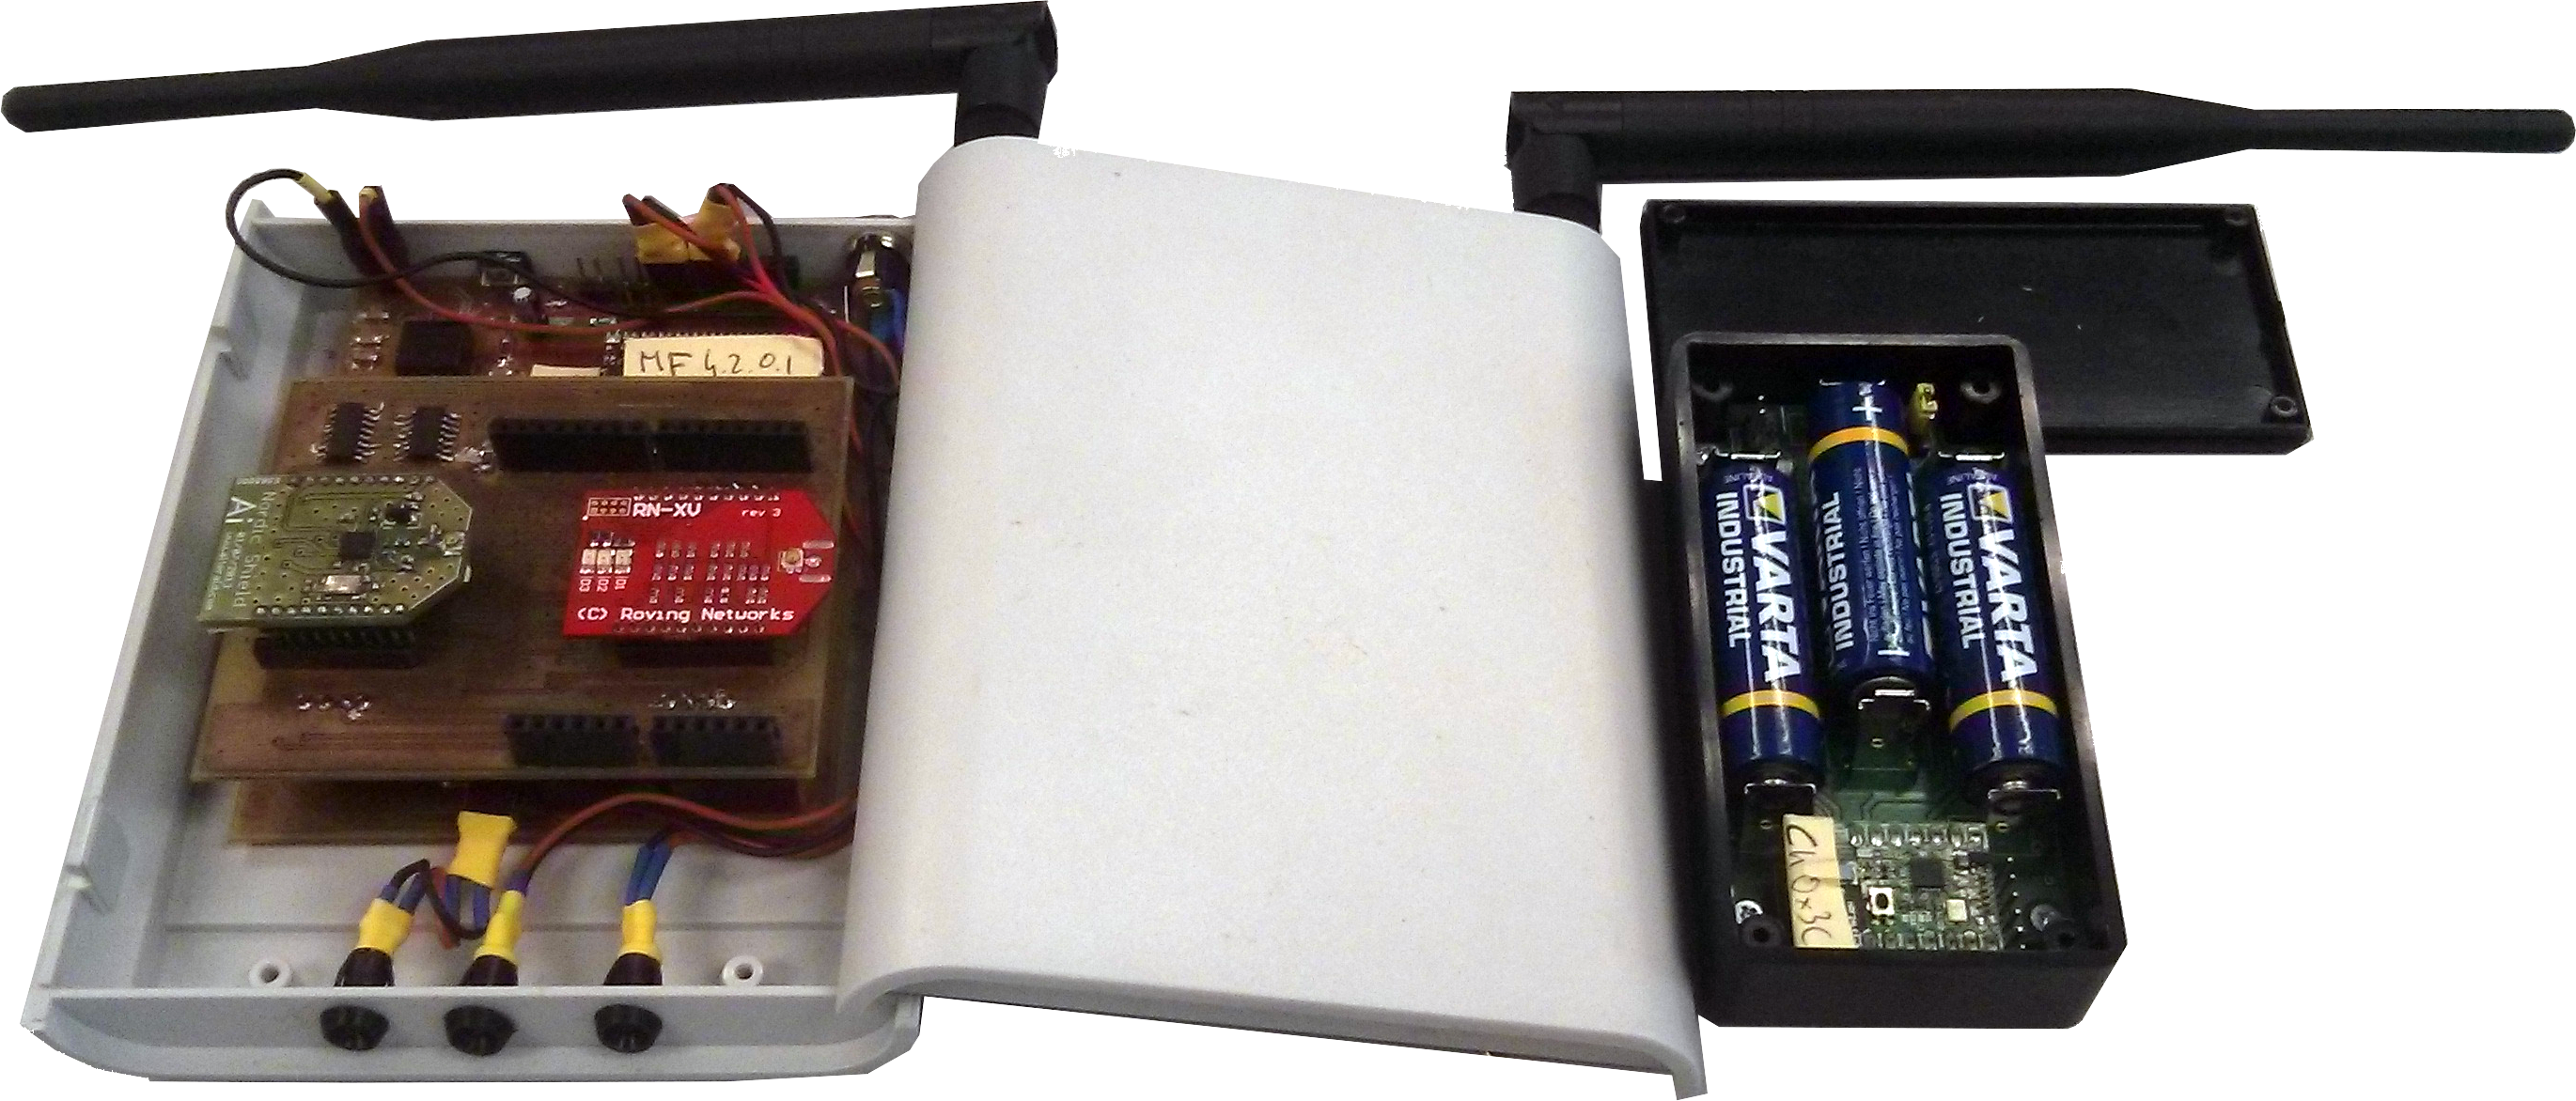
\includegraphics[width=0.7\textwidth]{pictures/proposal/homesense}
  \caption{Sensor on the left and HomeSense gateway on the right \label{fig:Proposal-HomeSense}}
\end{center}\end{figure}

\section{AlterNative}\label{S:Proposal-AlterNative}
AlterNative is a language translating tool created by Alex Albal\'{a} and Juan L\'{o}pez. It can translate a compiled (.NET) assembly or library to standard C++ code. Basically this program decompiles the file to be translated, then it sketches how the program works, which are its classes, functions, nodes, etc and then start translating step-by-step all the program. After that, it links the necessary C++ libraries to work, ones are from boost library, and the other ones are self-written to behave like the original C\# classes.
\\
It is interesting to emphasize that the main difference of this translator between the other existing ones is that it tries to generate a code practically identical to the original C\# source code. By doing this, the resulting C++ source is really easy to read for people not used to C++ syntax and language.
\begin{figure}[H]\begin{center}
 \centering
  \captionsetup{justification=centering}
 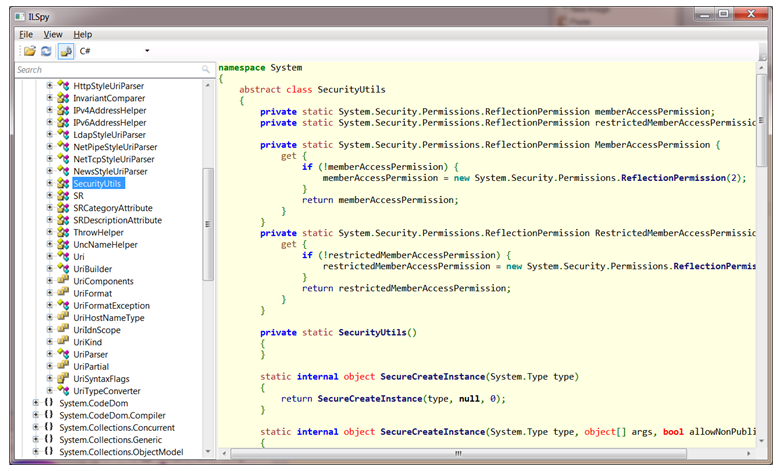
\includegraphics[scale=0.65]{pictures/proposal/alternativeUI}
  \caption{AlterNative interface \label{fig:Proposal-AN}}
\end{center}\end{figure}

\section{Thesis Proposal}\label{S:Proposal-Thesis-Proposal}
After introducing HomeSense and AlterNative is time to explain the thesis proposal itself because it is related to the applications mentioned above. The proposed project is to take the code of the HomeSense gateway, which is written using Micro Framework, and make it run in a Linux device instead of a Netduino Mini because it is getting limited in terms of capabilities, performance and expansion for future characteristics.
\\
The idea is to take the gateway code and port it to other devices capable of use minimum GPIO, interrupts from this ports, the SPI communication protocol and UART because all of them are used in the HomeSense source code. It is important to point that the implemented classes must be similar to the Micro Framework code to avoid major changes on the HomeSense program. Minor changes such as port renaming and communication module name changing are acceptable because they do not alter the original execution flow and design architecture. But not only this should be done on HomeSense, it is interesting to make portable between different hardware platforms any code that runs over Micro Framework.
\\
After accomplishing with this first goal, the second part of the thesis is to use AlterNative to translate the IOSharp library to C++ in order to increase and analyse the performance of IOSharp running on C++ instead of C\#. To accomplish with this objective, some C++ libraries must be written in order to translate IOSharp.

\subsection{Objectives}\label{SS:Proposal-Objectives}
The proposed objectives are listed below explaining briefly each one:  
\begin{itemize}
	\item \textbf{IOSharp:} objectives to be accomplished during the first part of this thesis.
		\begin{itemize}
		\item \textbf{GPIO:} Simple I/O functions (Input, Output ports).
		\item \textbf{Interrupts:} enable interrupts through GPIOs.
		\item \textbf{SPI:} get a working SPI bus on the implementation.
		\item \textbf{UART:} get a functional SerialPort
		\item \textbf{HomeSense:} deploy this WSN as a functional test to show the correct function of the library.
		\end{itemize}
	\item \textbf{AlterNative:} second part of the thesis involving the code translation tool.
		\begin{itemize}
		\item \textbf{Cross-Platform:} although one of the goals of AlterNative is produce a cross-platform source code, it only runs on Windows so Linux or MacOSX use are unable to use this tool because of the graphic dependencies. In this case, the code must be analysed and modified to produce a cross-platform program.
		\item \textbf{Library:} write the necessary methods to let IOSharp be translated.
		\item \textbf{Tests:} write functional tests to determine the correct functionality of the library.
		\item \textbf{Performance analysis:} do some performance analysis to check the performance increase when the code is translated.
		\item \textbf{Translate HomeSense:} do a complete translation of the WSN platform using AlterNative.
		\end{itemize}
\end{itemize}


\section{Document Structure}\label{SS:Proposal-Doc-Structure}
This document is structured on seven chapters that shows the project definition when this thesis was proposed, then a state of the art shows the current technologies or systems that are similar to this thesis. Then the development steps are enumerated where GPIO, interrupts, SPI and UART are involved. Another chapter is dedicated to the functional tests to proof that the IOSharp proposed objectives where done. After these tests an introduction to AlterNative is done along with the performance tests chapter which shows the results for the AlterNative part. Finally, the conclusions chapter summarizes the thesis.
\chapter{State of the art}\label{C:State-Art}

This chapter sketches out briefly the state of the art of the embedded operating systems and its capabilities. Then according to this thesis it will be explained what is the current operating system running on bottom of HomeSense and finally why has been chosen the RaspberryPi as the target device.

\section{Embedded Systems}\label{S:Embedded-Systems}
Embedded Systems now a days are taking relevance again with the Internet of the Things, environment sensing, Wireless Sensor Networks and all new coming technologies that require low power consumption, small size, mobility environments, ...

In Embedded Systems or Resource Constrained Systems it is interesting to take a look into the Hardware platform and its capabilities, the differences between platforms, and also which tools or unique features offers to developers.

An operating system (OS) offers an interface with the hardware to make it independent from the applications that the device runs, making easy the interactions between hardware and the programs running on the machine.

An OS is an important program that makes easy to develop applications, but it is important to maintain the features that the processor offers, avoiding performance or capabilities degradation. 
This bachelor thesis is focused on constrained-resource devices, where the processing capabilities and memory resources are limited, is fundamental to respect the above criteria.

\subsection{Operating Systems Architectures}\label{Operating-Systems-Architectures}
In general, there are three types of operating system architectures for embedded devices, which are based on how applications are executed or included into the OS.

\begin{itemize}
\item \textbf{Monolithic:} The OS and the applications are combined into a single program. Normally in this situations the embedded device runs in the same process the OS and the program written to it. This type of architecture makes difficult to include new functions without rewriting much of the code.

\item \textbf{Modular:} The OS is running as a standalone program in the processor and has de ability to load programs to it self as modules. In terms of the development, it's possible to develop applications without writing in the core of the OS. Normally using modules developers can expand the capabilities of its software.

\item \textbf{Virtual-Machine:} The OS creates an abstraction layer of its underlying hardware, this abstracted layer is common in every device that implements that virtual-machine. Using this type of operating system provides a helpful tool to achieve the well known slogan \textit{write once, run anywhere}. Although using virtual-machine devices simplifies the development on multiple devices, the performance of the platform normally will be reduced and in Real Time environments it isn't recommended to use it.
\end{itemize}

\subsection{Embedded Operating Systems}\label{Embedded-Operating-Systems}
There is a wide range of Embedded Operating Systems each of them has strengths and weaknesses, below different OS are described and compared.
 
\begin{itemize}
\item \textbf{TinyOS} is a popular open source OS for wireless constrained devices, many of them used in wireless sensor networks. It provides software abstractions from the underlying hardware. It is focused on wireless communications offering stacks for 6LoWPAN and ZigBee. It also supports secure networking and implements a RPL taking in mind the forthcoming routing protocol for low power and lossy networks.
\\
However, TinyOS changes how programs should be developed, it intended to use non-blocking programming which means that it isn't prepared for long processing functions. For example, when TinyOS called to send a message the function will return immediately and after a while the send will be processed and after then, TinyOS will make a callback to a function, for example send()'s callback will be sendDone().

\item \textbf{FreeRTOS} is a free real-time OS that supports over 34 architectures and it is being developed by professionals under strict quality controls and robustness. Is used from toys to aircraft navigation and it is interesting for its real-time qualities. It has a very small memory footprint (RAM usage) and very fast execution, based on hard real-time interruptions performed by queues and semaphores. Apart from this, there are not constraints on the maximum number of tasks neither the priority levels that can be used on tasks. 

\item \textbf{Contiki} is similar to TinyOS in terms of portability between platforms and its code is open source. It also offers features similar to standard operating systems like threading, timers, file system and command line shell and uses modular architecture, loading or unloading programs from its kernel. Contiki is build on top of the Internet Standards supporting IPv4 and IPv6 and also the new low-power internet protocols which includes 6LoWPAN, RPL and CoAP.
\\
Contiki uses protothreads which are designed for event-driven systems running on top of constrained devices, which is the case of Contiki's kernel. It provides blocking without having a real multi-threading system or a stack-switching.

\item \textbf{Micro Framework .NET} is a solution provided by Microsoft for constrained devices which cannot execute the full .NET stack. It is Virtual-Machine based operating system that a small implementation of the CLR making available to execute a small set of .NET classes. Its memory footprint is about 300KB and supports the common embedded peripherals like EEPROM, GPIO, SPI, UART, USB, ...
\\
One of its interesting features is that offers the advantages of .NET language using Visual Studio and it also offers real-time debugging directly on the device.
\end{itemize}



\section{Micro Framework .NET}\label{S:MicroFramework-dotNet}
MicroFramwork, is also known as NETMF, had its roots in a project called \textbf{Smart Personal Objects Technology (SPOT)}. The first devices implementing the SPOT technology where smart-watches from Fossil and Suunto in 2004 and after them became kettles, weather stations and for traffic and map updates in Garmin devices. Microsoft wanted to create a technology for everyday devices so they launched together with SPOT the MSN Direct which was a set of network services capable of delivering information to the SPOT devices using FM radio broadcast signals.
\\
In 2008 the production of SPOT watches was discontinued and in 2009 Microsoft released the source code of Micro Framework under Apache 2.0 license making availably to the community and shortly after this release the MSN Direct services where ceased.

\subsection{Devices using Micro Framework}\label{SS:MicroFramework-Devices}
Since Microsoft released the Micro Framework source code, different companies had created different devices supporting .NET code and this stack.
\\
There are two major vendors producing chips and development kits for this software. Secret Labs produces the netduino family which consists of the standard netduino, a netduino plus which is an enriched version. This one has better processor and memory, it includes an ethernet port and uses micro sd cards to provide storage. One of the interesting this of this two boards is the layout of the board, it is totally compatible with most of the arduino shields in the market.
Secret Labs has another board called netduino go, which is similar to netduino plus but without storage, ethernet and it does not use the typical arduino layout, so a globus module is required to use arduino shields.
\\
GHI Electronics is another hardware manufacturer that has designed and released different boards implementing Micro Framework or modules which its target platform is Micro Framework. GHI has a very wide range of products for example FEZ Cerbuino Bee and FEZ Cerbuino NET which are similar to the netduino plus in terms of performance. One interesting thing of FEZ devices over netduino is the possibility of load native code (C/Assembly) for real-time requirements which it is really interesting. For example HomeSense could run its Mesh driver in C and perform better than it performs using C\#.
\\
\\
In addition to the mentioned manufacturers, Microsoft Research in Cambridge has defined a hardware reference platform called .NET Gadgeteer which defines how boards and modules must be in order to allow rapid prototyping of projects. Gadgeteer boards and modules share the same layout and connector schemes and are open to any company that wants to build products using those schematics.

\subsection{NETMF on Linux}\label{S:NETMF-Linux}

After doing some research about implementations of Micro Framework on other devices or running on top of other operating systems such as Linux. It was found a project that is currently porting NETMF to Linux, but for a very specific device called Eddy.
\\
Eddy is an ARM embedded device board which uses Linux, the port named above has been made as a demonstration of writing NETMF applications using a port on top of other operating systems. One of the majors problems of this port is that some drivers are not working at all, for example UART, SPI and I2C which are 3 interesting I/O protocols and ports for HomeSense.
\\
Although this port is for the Eddy board, it can be ported to other devices using the appropriate cross-toolchain, anyway it seems that there is a lack of possibilities to run Micro Framework code in other devices or operating systems.

\subsection{NETMF on RaspberryPi}\label{S:NETMF-RPI}

If it is hard to find an implementation of NETMF in Linux it will be harder to find an implementation for RaspberryPi. In other words, people in GHI forums are asking for NETMF ports for RaspberryPi but no one exists.
\\
aqui nombrar altres implementacions en C# que acostumen a ser bastant escaces també


\section{Micro Framework in other devices}\label{S:NETMF-and-RaspberryPi}
Before starting with the development a search was done in order to know if there was any project involving the port of the MicroFramework to Linux devices using, for example, Mono. Nothing was found.
There is currently one implementation of MicroFramework for Linux, but it only works in a resource-constrained device called Edy Linux.

RaspberryPi has many implementations in different languages involving its IO ports, many are written in C and Python, others are for example in Java. But when speaking in terms of .NET/C\# there is an important lack in IO implementations, below are exposed the most important ones that where found.

\begin{itemize}
\item \textbf{BlaBlaBla:}
\item \textbf{BlaBlaBla:}
\end{itemize}

Although the XXX library is really interesting according to it's description of functionality, it doesn't 


\chapter{State of the art: Embedded Operating Systems}\label{C:State-Art-Microframework}

This chapter sketches out briefly the state of the art of the existing operating systems for embedded devices. The first part enumerates the different operating systems, explaining its important features. Next, focusing on MicroFramework, the different devices will be listed, which ports exist and finally, the existing implementations to use the Input/Output ports on a RaspberryPi.

\section{Embedded Operating Systems}\label{S:Embedded-OS}

An operating system (OS) offers an interface with the hardware to make it independent from the applications that the device runs, making easy the interactions between hardware or other running programs.

An OS is an important program that makes easy to develop applications, but it is important to maintain the features that the processor offers, avoiding performance or capabilities degradation. As this bachelor thesis is focused on constrained-resource devices, where the processing capabilities and memory resources are limited, is fundamental to respect the above criteria.

In general, there are three types of operating system architectures based on how applications are executed:

\begin{itemize}
\item \textbf{Monolithic:} The OS and the applications are combined in a single program, being an end to end task without the possibility to include new functions without rewriting much of the code.

\item \textbf{Modular:} The OS is running as a standalone program in the processor and has de ability to load programs to it self as modules. In terms of the development, it's possible to develop applications without writing in the core of the OS.

\item \textbf{Virtual-Machine:} The OS creates an abstraction layer of its underlying hardware, this abstracted layer is common in every device that implements that virtual-machine. Using this type of operating system provides a helpful tool to achieve the well known slogan \textit{write once, run anywhere}. 
\end{itemize}


\begin{itemize}
\item \textbf{TinyOS:} asdf asdf asdf.

\item \textbf{FreeRTOS:} asdf asdf asdf.

\item \textbf{uC/OS II:} asdf asdf asdf.

\item \textbf{Contiki:} asdf asdf asdf.

\item \textbf{Micro Framework .NET:} asdf asdf asdf.
\end{itemize}



\section{Micro Framework .NET}\label{S:MicroFramework}

Complexity and heterogeneity drawbacks of distributed systems could be solved or relived using a middleware. Middleware is a system software that resides between the applications and the underlying operating systems, network protocol stacks, and hardware, which provides facilities in order to build and use distributed systems \cite{cite:middleware}.

This type of software provides a transparent and abstract vision of the low-level details (e.g. network communication, encoding, concurrency, protocol handling, etc.) facilitating end user programming. Middlweware typically provides two different types of transparency to distributed systems:

\begin{itemize}
\item \textbf{Access transparency:} Hides differences between remote and local operations like data representation and invocation mechanisms.

\item \textbf{Location transparency:} Hides where the components reside. The  different components could be 
redistributed (e.g. moved between computers) without changing any of the other components.
\end{itemize}

\subsection{NETMF enabled devices}\label{SS:MicroFramework-Devices}

MicroFramework can run on CLR enabled devices that are MicroFramework compilant with it's specifications. In this bachelor thesis a Netduino Plus (from XXXXXLabs) has been used to test, understand and code sample code in order to know how Microframework works. Apart from this Netduino there are other devices like the cerbuino,which are also capable to run CLR code.

Among this, there are more powerful devices that can run and execute simple graphics programs.


\subsection{Software Development Kit}\label{SS:MicroFramework-SDK}
As Micro Framework is similar to an operating system it has

\begin{itemize}
\item \textbf{4.3:} This asynchronous indirect communication model uses a queue in order to exchange messages. The messages from the producer are stored into the consumer's queue after being sent. In this type of model, persistent queues are used when the reliability is required in front of performance. Quality of service (QoS) policies are also a good solution to provide reliability.

\item \textbf{4.2:} In this direct communication model, the messages are sent directly to the interested parts through publish/subscribe pattern. In this pattern, the different parts register interest in receiving messages on a particular message topic. After the subscription, the consumer will receive any message corresponding to the subscribed topic.

\end{itemize}

BlaBlaBla both blablabla

\subsection{Visual Studio}\label{SS:MicroFramework-IDE}

\section{RaspberryPi and MicroFramework}\label{S:RaspberryPi-NETMF}
Before starting with the development a search was done in order to know if there was any project involving the port of the MicroFramework to Linux devices using, for example, Mono. Nothing was found.
There is currently one implementation of MicroFramework for Linux, but it only works in a resource-constrained device called Edy Linux.

RaspberryPi has many implementations in different languages involving its IO ports, many are written in C and Python, others are for example in Java. But when speaking in terms of .NET/C\# there is an important lack in IO implementations, below are exposed the most important ones that where found.

\begin{itemize}
\item \textbf{BlaBlaBla:}
\item \textbf{BlaBlaBla:}
\end{itemize}

Although the XXX library is really interesting according to it's description of functionality, it doesn't 
%\chapter{MAREA}\label{C:MAREA}

\textcolor{red}{//TODO}

\section{Description}\label{S:MAREA-description}

Middleware Architecture for Remote Embedded Aplications (MAREA) is a middleware designed by ICARUS group specifically designed to fulfil Unmanned Aircraft Systems (UAS) communications and their application to the design of complex distributed UAS avionics \cite{cite:marea}.

The ICARUS group is composed by researchers of the Polytechnic University of Catalonia - Barcelona Tech (UPC) mainly from the Computer Architecture Department of the Castelldefels School of Telecommunications and Aerospace Engineering (EETAC). The basic aim of this research group, formed in 2005, is develop technologies to automate air traffic management (ATM) with low cost UAS in civil airspace.

MAREA proposes a modular architecture based on services (SOA).These type of architectures ensures extensibility, flexibility and interoperability across heterogeneous environments. MAREA is a MOM implements a Data Distribution System communication model based on the publish/subscribe pattern. This middleware also offers additional features like RPC and file-based data transfer. 

\section{Communication primitives}\label{S:MAREA-primitives}

MAREA provides to the developers a different range of possibilities to interact and communicate the services between them through the following communication primitives:

\begin{itemize}
\item \textbf{Variables:} This type of communication primitive is designed to share periodic and short deterministic information between different services following a publish/subscribe model. In this type of primitives the data is sent in a best effort way, through UDP transport, taking in account the periodic behaviour of the publisher and the limited lifetime of the information. An appropriate use case of this type of primitive is the telemetry provided by a GPS navigation device.   

\item \textbf{Events:} Similar to the variables, events are also used to share periodic and short information between services following a publish/subscribe model. As opposite of variables, the information in events is guaranteed to be delivered to all the subscribed services through TCP transport. This type of primitive is designed to share information about important and unpredictable facts. An example of this type of communication primitive can be any alarm used to inform about a critical system failure. 

\item \textbf{Remote invocation:} MAREA also offers an alternative Data Distribution System communication model to the publish/subscribe pattern like remote invocation. In this type of primitive the communication is established only between two services following the request/reply pattern using a client/server model. In remote invocation, as opposite of variables and events, the relation between the two services is punctual and it only lasts the execution time of the remote call. This type of primitive allows the use of multiple parameter and a single result value. Remote invocation is useful in these situations where an one-off action has to be taken.

\item \textbf{File-based data transfer:} This type of communication primitive is used to transfer continuous 
information in a efficient way. In file-based data transfer the information is sent in chunks in a non reliable way through UDP Transport. File-based data transfer also provides a reliable control mechanism in order the consumer could notify the missing packets to the provider. This type of communication primitive is useful to share any kind of information like images and configuration files.
\end{itemize}

\section{System architecture}\label{S:MAREA-architecture}

As shown in figure \ref{fig:marea-system-architecture} MAREA has been designed according to the following three layer system architecture: transport, encoding and protocol. One of the purposes of this design is to provide flexibility allowing the use of different transports and encodings depending on the circumstances (e.g. hardware and software limitations).

\begin{figure}[H]\begin{center}
 \centering
  \captionsetup{justification=centering}
  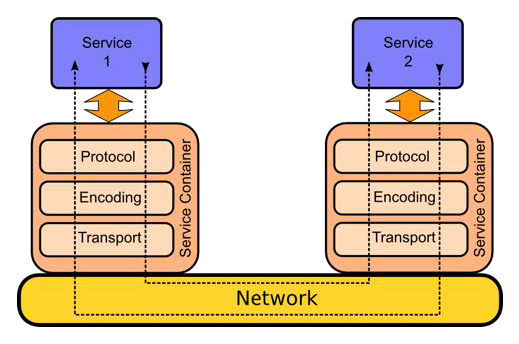
\includegraphics[scale=1]{pictures/marea/Architecture}
  \caption{A high level view of Marea middleware layers. The figure shows two MAREA containers with their internals layers: Protocol, Encoding and Transport  \cite{cite:thesis-soa-avionics} \label{fig:marea-system-architecture}}
\end{center}\end{figure} 

For one hand, the main aim of the encoding layer is to translate MAREA protocol messages in streams on bytes and also take the inverse operation. For the other hand, the transport layer, as it names suggests, is on charge transfer data (streams of bytes) through the network. From now to the end of the document, these two layers are also referenced as one single layer called network layer. The design and implementation details of these two layers are explained in chapter \ref{C:NetworkLayer}.

The protocol layer is responsible of manage and process MAREA protocol messages. This layer also controls and manages the exchange of these messages in order to discover, publish and subscribe the different services.

These three layers are controlled by the main component of the middleware which is called service container. This element allows message passing between the services, controls local and remote services, manages the communication primitives, etc. The service container makes the middleware layers transparent and decouples the services from the core of the middleware.

\section{Naming service}\label{S:MAREA-naming} 

The naming service allows MAREA to find, share and access services and its communication primitives hiding the network complexity. This component should address the different service and its communication primitives by name resolution. 

An important requirement of the naming service is that the resolution name should not be bounded statically to specific locations. The main problem with that is if the service is moved to another location the reference to it becomes invalid. The proposed solution to this problem is use location independent service identifiers.

The URL expression is a string comprising five fields separated by a slash which correspond to four different hierarchical levels. Each of the fields represent a hierarchical level name space, with exception of the service and the primitive are in the same level. The information of this four hierarchical levels is represented following the following format:

\begin{center}

/<subsystem>/<node>/<instance>/<service>/<primitive>
\end{center}

\begin{itemize}
\item \textbf{Subsystem:} A subsystem is defined as a logical group of nodes.  
\item \textbf{Node:} A node is defined as a group or just a single processor which runs the middleware.
\item \textbf{Instance:} The instance identifies the different instances of a service.
\item \textbf{Service:} The service identifies the type of the service.
\item \textbf{Primitive:} The primitive identifies a specific communication primitive.
\end{itemize}

The naming scheme allows the usage of special characters in each of the hierarchical levels to provide flexibility to the service location. The table \ref{T:Marea-Naming-Char} shows a brief description of each of one.

\begin{table}[H]
\begin{center}
\caption{\nohyphens{MAREA naming special characters}}
\label{T:Marea-Naming-Char}
\begin{tabular}{|l|p{7.3cm}|l|}
\hline
 {\bf Special character} & {\bf Description} & {\bf Usage} 										\\ \hline \hline
 * & Selects any element of the actual field/hierarchical level & Any of the fields of the URL\\ \hline
 ! & Locks the service with highest priority of the set referenced by the URL & At the beginning of the URL\\ \hline
 \# & Forces static name resolution for the given URL & At the beginning of the URL \\ \hline
\end{tabular}
\end{center}
\end{table}

For instance, /Vehicle 1/Devices/*/GPS means all the GPS type instances in the node Devices belonging to subsystem Vehicle 1, regardless of their instance name. /Vehicle 1/*/*/* means all the services of Vehicle 1.

MAREA presents by default dynamic name resolution. This means that if a new service is started, the naming service is able to notice it and update all the name resolutions which contain a reference to this service.

In some specific cases its required the use of static name resolution. In these situations the changes will not be taken into account to accomplish the name resolution.

\section{Service description}\label{S:MAREA-services}

\textcolor{red}{//TODO}
%\chapter{Network Layer}\label{C:NetworkLayer}

The first part of this chapter presents the new network system architecture and compares it with previous one.

The following subsections describe each of its main components and present results in order to measure and compare the performance with the old design. The key performance parameters analyzed depending on the architecture component are: simultaneous connections, round-trip time (RTT) and memory allocation.

\section{Architecture}\label{S:Architecture}

The network layer is the lowest level layer on the MAREA stack. This layer it is on charge of provide an optimized, modular and reusable usage of the network capabilities. MAREA network system architecture consist of two main sublayers: encoder and transport.

%width=\linewidth
\begin{figure}[H]\begin{center}
 \centering
  \captionsetup{justification=centering}
  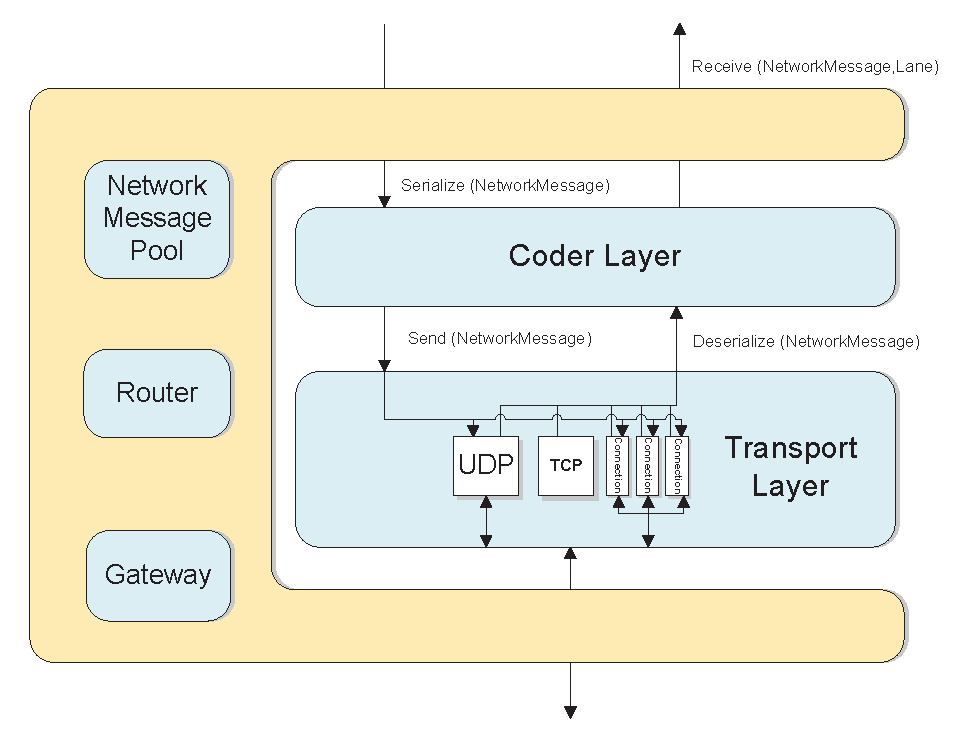
\includegraphics[scale=0.8]{pictures/network/Network}
  \caption{MAREA 2 network layer architecture \label{fig:network-architecture}}
\end{center}\end{figure}

One one hand, the encoder layer is responsible of code MAREA protocol messages into byte sequences. This component also undertakes the inverse operation of decode byte sequences into MAREA protocol messages. 

On the other hand, the transport layer is on charge of send and receive data (byte sequences) from the underlying network through different types of transports (UDP, TCP).

The idea of the proposed design, in order to improve the performance in terms of speed,  is to minimize the amount of time used by the garbage collector to create and destroy object instances.  The architecture component called NetworkMessage pool achieves this improvement using a memory pool mechanism.

The network layer is a highly reconfigurable system that allows the use of different types of encoders and transports. The router is the main component that select this components dynamically. This module it also can be configured by the user of the middleware depending on the scenario.  

The gateway module is on charge of interconnect networks that use different types or protocols and architectures. Its main goal is the translation of the source network protocol to the destination network protocol, and vice versa, in order to allow the communication between them.

In order to provide uniformity and simplicity to the design of each sublayer, the communication between them is done using a common interface. Each of the sublayers send and receive a NetworkMessage entity (figure \ref{fig:network-message}) to the upper and lower layers. This common data structure, which contains all the necessary information used by the encoding and transport layers, is modified as it travels downward or upward the architecture. 

\begin{figure}[H]\begin{center}
 \centering
  \captionsetup{justification=centering}
  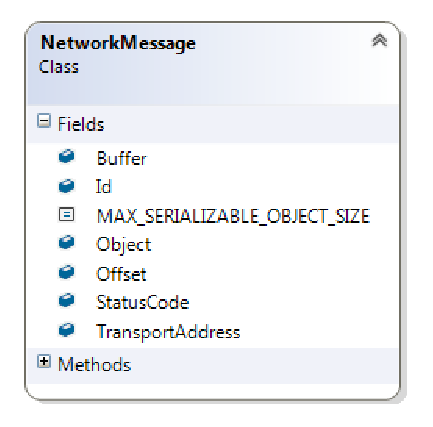
\includegraphics[scale=0.75]{pictures/network/NetworkMessage}
  \caption{NetworkMessage entity \label{fig:network-message}}
\end{center}\end{figure}

One one hand, when encoder sublayer serializes a MAREA message (which is actually stored in the field Object of the NetworkMessage entity), the resulting byte stream is saved in the Buffer field. At the same time, the total length of the serialized data is assigned to the field Offset.

On the other hand, the deserialized incoming MAREA messages are stored in the field Object according to the byte stream and the length of the received data provided by the transport sublayer (this information is contained in the fields Buffer and Offset respectively). 

In relation to the transport layer, when a message is received the fields StatusCode and TransportAddress are set in order to inform the upper layers about the reception status and the source of MAREA message.

\subsection{Comparison with MAREA 1 Network Architecture}\label{SS:Comparison-with-MAREA-1-Network-Architecture}

One of the main differences between the old and new MAREA network designs is the top entry point of the architecture which is called Lane manager. This component is the responsible to control which transports and encoders are used by the middleware at a particular moment. In contrast, the router is the responsible of perform this task in the new architecture.

%width=\linewidth
\begin{figure}[H]\begin{center}
 \centering
  \captionsetup{justification=centering}
  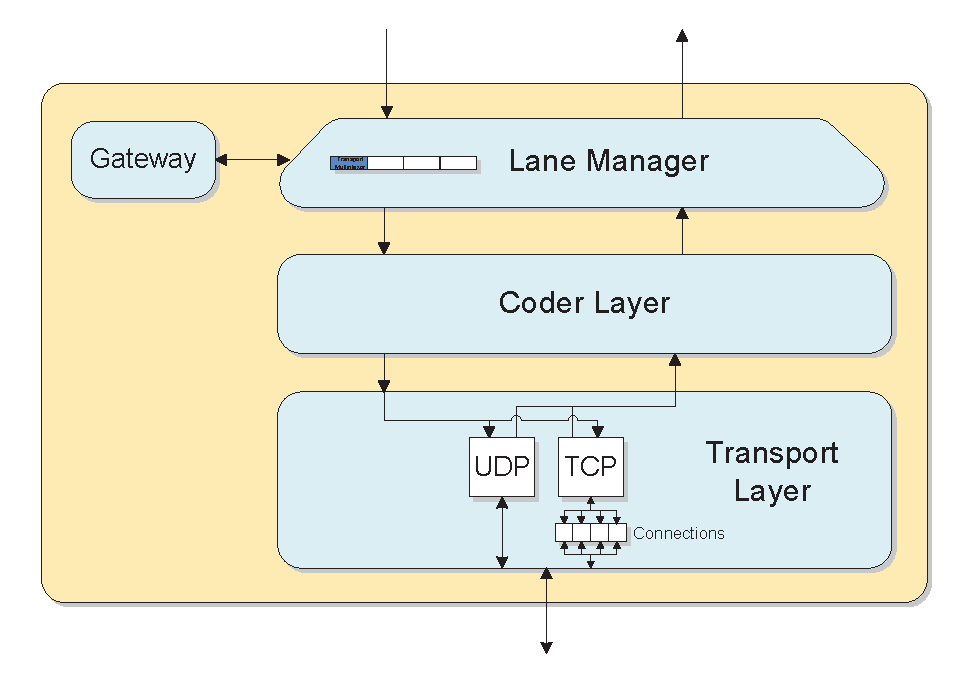
\includegraphics[scale=0.8]{pictures/network/NetworkOld}
  \caption{MAREA 1 network layer architecture \label{fig:network-old-architecture}}
\end{center}\end{figure}

As opposite of the new architecture, network lanes (subsection \ref{SS:Network-Lanes}) are not a set of references to the bindings establish between the different network architecture elements. Instead of this, there are object references (copies) to these elements.

The main idea of taking out the Lane manager in the new architecture is to simplify the design and improve the speed by removing unnecessary repeated searches to the lane, which in normal conditions is always the same. Every time a message is sent in MAREA 1 network architecture, a search has to be done into dictionary in order to get the default lane.

\begin{figure}[H]\begin{center}
 \centering
  \captionsetup{justification=centering}
  
\includegraphics[scale=2]{pictures/network/LaneManager}
  \caption{Lane manager class diagram \label{fig:lane-manager}}
\end{center}\end{figure} 

The new design does not use a dictionary in order to avoid slowdowns in the performance. Instead of this, the network layer use only one output and input lane for the outgoing and incoming data respectively. This lanes are reused while the network continues to work properly. 

The service container, which is the immediate upper layer, is the responsible of keep and provide the hint to the network layer every time. Only if a network change happens, new lanes are demanded to the router. This solution is more complex but reduces the acquisition time of the lanes.

In the transport sublayer, lanes also take profit of its new approach by taking reference directly to the TCP connection which is required in a particular moment instead of searching it in a dictionary.

Another big difference between the two architectures is the sublayer architecture design. For one hand, the MAREA 2 network sublayers (figure \ref{fig:network-architecture}) are uniform. In MAREA 1 the network sublayers (figure \ref{fig:network-old-architecture}) are inconsistent because every single sublayer presents different interfaces in order to communicate with to the upper and lower sublayers. 

For the other hand, in the old architecture every sublayer is dependent of the upper and lower one because it has to keep a reference in order to communicate with them. The new sublayer architecture is more independent and flexible, because the responsibility of manage the bindings between the different sublayers is delegated to the network lanes instead of the sublayers by itself.

Another difference, that has been mentioned before, is the pooling mechanism used in the new architecture which is explained in section \ref{S:Network-Message-Pool}.

\section{Router}\label{S:Router}

MAREA is able to use different encoders and transports in order to to build a modular and configurable network architecture. The router has the ability to select the elements (encoders and transports), of the layered network architecture, at execution time depending on needs and the state of the network. The main aim of this element is to create and manage the network lanes.

\subsection{Network Lanes}\label{SS:Network-Lanes}

A network lane can be defined as a set of references to the bindings establish between the different network architecture elements (encoder and transports) used at a particular moment. Lanes have been implemented as linked lists of delegates or multicast delegates. A delegate is an object that allows the programmer to encapsulate a reference to a method (but is similar to a function pointer in C or C++ but is object-oriented, type-safe, and secure) \cite{cite:delegate}.

The following characteristics of multicast delegates have been taken in account to create network lanes:

\begin{itemize}
\item The invocation list of multicast delegates is called synchronously and orderly.
\item If an exception occurs in a delegate, the remaining delegates of the list are not invoked.
\end{itemize}

According to the figure \ref{fig:network-message} the router use at least two different network lanes to send and receive data.

\begin{table}[H]
\begin{center}
\caption{\nohyphens{Output and input network lanes}}
\label{T:Lanes}
\begin{tabular}{|l|p{7.3cm}|}
\hline
 {\bf Lanes} & {\bf Invocation List} 												\\ \hline \hline
 Output Lane & MareaCoder.Serialize(NetworkMessage m)\newline Transport.Send(NetworkMessage m)\\ \hline
 Input Lane & Coder.Deserialize(NetworkMessage m)\newline Container.Receive(NetworkMessage m)\\ \hline
\end{tabular}
\end{center}
\end{table}

A way to trap link loss or disconnection exceptions it is required in order to notify the upper layers that an error has occurred. There exist two different solutions to this issue:

\begin{itemize}
\item Use the method GetInvocationList to get each individual delegate from the multicast delegate and invoke each delegate within the try block of an exception handler. This solution is very powerful but it has counterparts like the use of system resources and execution time due to the handling of exceptions. 
\item Use a field in the NetworkMessage entity as a status code (figure \ref{fig:network-message}).
\end{itemize}

The second alternative has been implemented in order to accomplish with the objective of improve the performance. 

\section{NetworkMessage Pool}\label{S:Network-Message-Pool}

The non deterministic process of garbage collection is executed .NET virtual machine in order to maintain the memory clean. This process can introduce non deterministic pauses into the execution of a program which are not correlated with the algorithm being processed.

One solution in order to reduce garbage collection interruptions is use a memory pooling mechanism. The main idea of this type of mechanisms is to provide a managed set of functions in order to allocate and deallocate memory. The use of pooling mechanisms keep references to object instances that are beyond destruction, allowing it to be reused when needed. With this technique no objects (NetworkMessage entities) are released to be garbage collected until the middleware is shut down.

The proposed design to implement a memory pool mechanism is to use a FIFO queuing discipline for NetworkMessage entities. In this common queue disciple, the elements are added to the tail are removed from the head using a pair of object references to the tail and the queue.

The final purpose of the NetworkMessage pool is to reduce the amount of work that has to be done by the garbage collector in order to minimize the time used by its own execution. 

\subsection{Results}\label{SS:Network-Message-Pool-Results}

A memory allocation profiling test has been executed in order to evaluate the behavior of the NetworkMessage pool. The figure \ref{fig:pool-memory-allocation} presents the total bytes allocated by MAREA 1 and the MAREA 1 network backport (section \ref{S:MAREA-1-Network-Backport}) during a echo request/response test with two MAREA instances. Each instance runs a different service which sends or responds to the messsage. This results correspond to the total bytes allocated by the sender.

The test has been executed 100000 times to send variables (UDP) and events (TCP) primitives with a total payload of 1000 bytes and frequency of 100 Hz. MAREA 1 network backport has been tested in two different modes: reusing network lanes and creating every time on demand. 

\begin{figure}[H]\begin{center}
 \centering
  \captionsetup{justification=centering}
  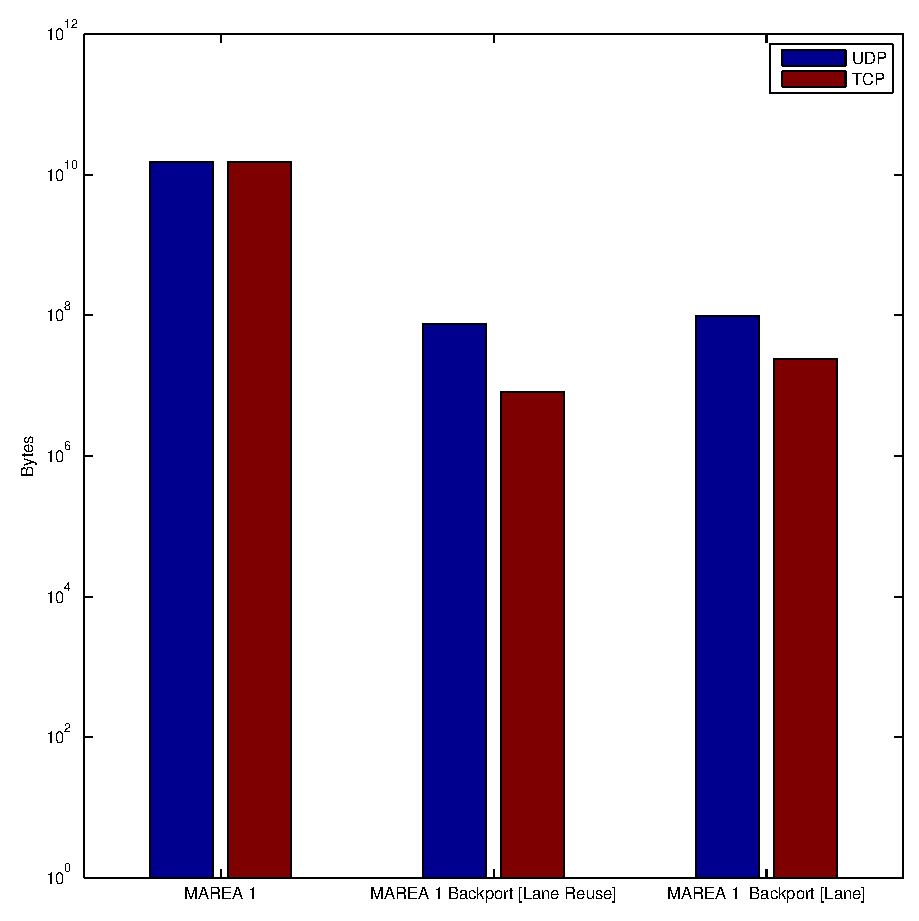
\includegraphics[scale=0.6]{pictures/network/MemoryAllocationBackport}
  \caption{Total bytes allocated in MAREA 1 and MAREA 1 network backport (1000 Bytes, 10000 packets, 100 Hz) \label{fig:pool-memory-allocation}}
\end{center}\end{figure}

\section{Encoding Layer}\label{S:Encoding-Layer}
The encoding layer is on charge of serializing and deserializing MAREA messages. This layer provides an abstraction layer such all logic above contained in the upper-layers does not need to know the particulars about how messages are serialize and deserialized.

Serialization is the act of taking an in-memory object or object graph (set of objects that reference each other) and flattening it into a stream of bytes \cite{cite:serialization}. The reverse operation is deserialization which takes a data stream and regenerates into an in-memory object or object graph.

\subsection{Previous Work}\label{SS:Encoding-Layer-Previous-Work}
The initial version of MAREA has been implemented with the idea of providing several encoding layer implementations (XML serialization, binary serialization and MAREA coder) in order to allow adaptability and interoperability between the devices and the network. The first two implementations of the encoding layer use .NET Framework serialization mechanisms such as binary serialization through BinaryFormatter class, and human-readable XML serialization through XMLSerializer class.

The BinaryFormatter is easy to use and automatic, but it is not such flexible as XMLSerializer. For the other hand XMLSerializer is slower and less powerful because it is not able to restore shared object references.  Furthermore, XML serialization does not convert private fields, indexers, methods, or read-only properties (except read-only collections). In order to do this, is mandatory to use the BinaryFormatter class.

\begin{table}[H]
\begin{center}
\caption{\nohyphens{Serialization engine comparison between .NET BinaryFormatter and XMLSerializer}}
\label{T:NetBinaryXML}
\begin{tabular}{|l|c|c|}
\hline
{\bf Feature} & {\bf BinaryFormatter} & {\bf XMLSerializer}          \\ \hline \hline
Level of automation                            & *****   & ****      \\ \hline
Type coupling                                  & Tight   & Loose     \\ \hline
Version Tolerance                              & ***    & *****      \\ \hline
Can serialize nonpublic fields                 & Yes   & No           \\ \hline
Preserves the object reference        		   & Yes   & No           \\ \hline
Suitability for interoperable messaging        & **    & ***         \\ \hline
Flexibility in reading/writing XML files       & -     & ****        \\ \hline
Compact output                                 & ****  & **           \\ \hline
Performance                                    & ****  & * To ***       \\ \hline
\end{tabular}
\end{center}
\end{table}

One of the main drawbacks of these two mechanisms is the performance overhead. Serializing a message with BinaryFormatter is expensive because of the metadata present. This is more noticeable in XMLSerializer because the overhead introduced by the XML tags is bigger. 

Another disadvantage of these two mechanisms is the interoperability between the different virtual machine representations of .NET Frameworks. For instance, XML serialization is not available on the Micro Framework and binary serialization works different in .NET Framework and .NET Compact Framework.

The last implementation of the encoding layer, which is called MAREA coder, has been designed in order to solve these two drawbacks controlling the serialization and deserialization of the different types. This technique, allows the programmer to have more control over the serialization and deserialization processes and ensures serialization compatibility.

The first implementation of this encoder was made using introspection to serialize and deserialize each message dynamically. The results of this first approach were not satisfactory in terms of speed because introspection it is a slow process. Custom serialization solves this issue by using specific methods or routines to serialize and deserialize specific MAREA messages.

MAREA coder has better performance in terms of speed and serialized data size than .NET BinaryFormatter and XMLSerializer implementations. MAREA coder is not dependent of the .NET Framework, so the interoperability between different virtual representations of the .NET Frameworks is not a problem like in .NET BinaryFormatter and XMLSerializer implementations.

\subsection{Drawbacks}\label{SS:Encoding-Layer-Drawbacks}
MAREA coder has some drawbacks inherited from custom serialization like complexity, especially in those cases like tree of objects or object graphs that might contain cycles. In these cases the code could be really hard to study. 

Another point that has to be taken in account of this approach is development speed. Custom serialization does take time for testing, developing and maintenance. For instance, if some messages are added or modified in the protocol layer, the corresponding methods to serialize and deserialize these messages must be added or modified too in order the encoder layer continues to work properly.

MAREA coder has been designed with two serialize and deserialize entry point methods that implement a large switch statement to get the type of object that has to be serialized/deserialized. A large switch statement means the method is large, hard to read and can generate very high complexity metrics.

\subsection{Improvements}\label{SS:Encoding-Layer-Improvements}
The following subsection presents an alternative design for the encoding layer in order to solve the drawbacks of MAREA coder.  

The new proposed design is based on an automatic tool called MAREAGen. This tool generates classes automatically with methods to serialize and deserialize MAREA entities marked as serializable. This eliminates the need for developers to implement serializing and deserializing code and guarantees run-time type safety.

Serialize and deserialize methods have been implemented as static because they have no instance. This type of methods is slightly faster than instance methods because are called with type name instead of an instance identifier. Serialize and deserialize methods also include inlining through the method implementation option agreessive inlining (Listing \ref{lst:SlowData}). This option allows compiler to eliminate the cost of method calls if it is possible. 

\begin{lstlisting}[caption={Class to serialize/deserialize MAREA SlowData messages },label={lst:SlowData}]
public class MG_SlowData
{
  /**
  * This static constructor is called by MAREA in order to load 
  * and register the identifier and specific methods to serialize
  * and deserialize this type.
  **/
  static MG_SlowData()
  {
    M2CoderTables.GetInstance().AddClass(typeof(Marea.SlowData), 50,
    MG_SlowData.Decode, MG_SlowData.Encode);		
  }

  public static readonly ulong MAREAGEN_FINGERPRINT= 11653293;
  
  /**
  * This method serializes all the different objects contained
  * inside a SlowData message into the given byte array.
  **/
  [MethodImpl(MethodImplOptions.AggressiveInlining)]
  public static void Encode(object theSlowData, byte[] buffer, ref int offset)
  {
    //Serialize fields...
  }

  /**
  * This method deserializes all the different objects of  a
  * SlowData message from the given byte array. This method also
  * returns the whole SlowData object 
  **/
  [MethodImpl(MethodImplOptions.AggressiveInlining)]
  public static object Decode(byte[] buffer, ref int offset)
  {
    SlowData slowdata = new SlowData();
    //Deserialize fields...
    return slowdata;
  }
}
\end{lstlisting}

MAREAGen provides fingerprints in each of every generated class, derived from the type definition, in order to provide an unequivocal and fast way to detect code that had not been recompiled. 

At the end of every execution, MAREAGen generates a XML and a DLL file which contains a list of the generated types with its unique byte code identifier and the generated classes to serialize and deserialize MAREA serializable classes respectively.

The proposed solution to solve the complexity issues is to include a hash table and a array of delegates for serialization and deserialization methods. Each of these collections also stores a reference to the byte code identifier provided by MAREAGen: the key values in case of the hash table and the index in case of the array)

One of the things that has to be accomplished in order to store the delegates into a dictionary is that all of the different serialize and deserialize methods must have a compatible signature (encode and decode methods from Listing \ref{lst:SlowData}).

With this approach, the complexity of having large methods with a lot of switch statements is reduced by moving each of the code sections, for every type of MAREA message, to a specific serialize and deserialize methods. 

Furthermore, the speed performance should be improved using the dictionary with the byte code identifiers, because with this solution long switch statements are avoided. The proposed approach is also more scalable: if the number of MAREA messages grows the serialization time should maintain constant, because it only depends on the time to access time to the delegates contained in the dictionary.

The table \ref{T:Messages-Id} presents the proposed byte code identifier distribution according to the different types used by MAREA Coder. MAREA protocol message identifiers are assigned at the beginning in order to reuse them in the service container. Similar to the encode layer, the service container has an array of delegates used to process each MAREA protocol message according to its identifier. In this case the position of the delegates inside the array correspond to the MAREA protocol message byte code identifier.

\begin{table}[H]
\begin{center}
\caption{\nohyphens{MAREAGen identifier distribution}}
\label{T:Messages-Id}
\begin{tabular}{|l|p{7.3cm}|}
\hline
 {\bf Id} & {\bf Type} 												\\ \hline \hline
 From 0 to 63 & MAREA protocol messages\\ \hline
 64 & Null\\ \hline
 From 65 to 126 & MAREA Coder basic types \\ \hline
 127 & Not null\\ \hline
 From 128 to 255 & MAREA Coder types created by MAREAGen\\ \hline
\end{tabular}
\end{center}
\end{table}

Once MAREA is started the DLL file generated from MAREAGen tool is used by MAREA coder in order to add the type code and delegates of the generated classes in the dictionary. This task is performed automatically, running the class constructor methods of classes that have been previously generated by MAREAGen.

Marea coder serialize and deserialize specific methods have also been modified in order to reduce the data size. For instance, the size of serialized System.Double is now reduced from 11 Bytes to 5 Bytes(1 of this 5 bytes is Marea  to encode the number 19 that indicates that the payload is a double).

Another new feature of this implementation is the support for some of the most commonly used  .NET collection types like lists, dictionaries and hash tables. 

The following bugs have also been resolved according to the results obtained in the implemented unit testing with NUnit tool:

\begin{itemize}
\item Compatibility with UTF8 character encoding.
\item Overflow exceptions for high values (double.MaxValue) in double types.
\item Support for run-time/dynamic Enum types.
\item Full support of polymorphic capabilities: Inheritance and control of null objects in object trees.
\end{itemize}
	
\subsection{Results}\label{SS:Encoding-Layer-Results}

The figure \ref{fig:coder-latencies} presents the total serialization and deserialization time for some specific types for the previous and the new implementation of MAREA coder. The most representative type is the specific MAREA message SlowData. This message is used by MAREA to transmit the data of the different MAREA primitives(variables, events, remote invocation, file-based data transfer). This time is 223.49 and 19.64 \textmu s for the old and new implementation respectively. Notice that the y axis in the figure is a logarithmic scale.

\begin{figure}[H]\begin{center}
 \centering
  \captionsetup{justification=centering}
  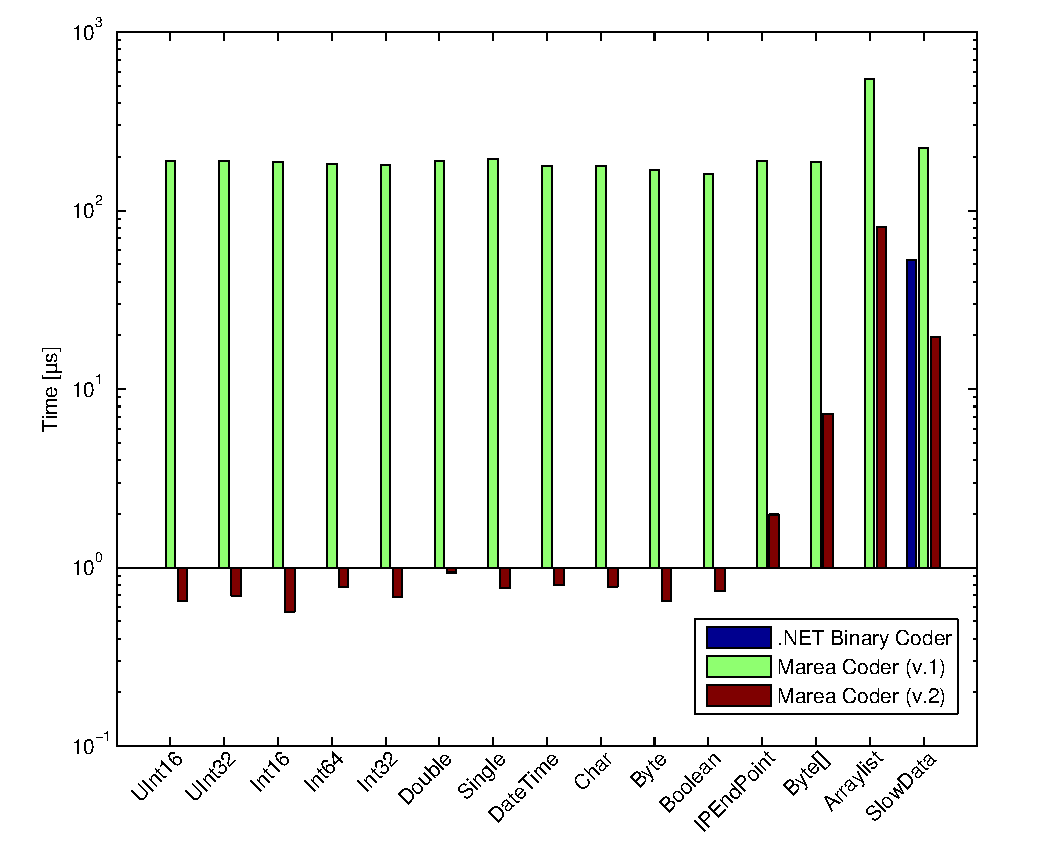
\includegraphics[scale=0.6]{pictures/network/LatencyCoder}
  \caption{Encoder layer implementations: Total serialization and deserialization time\label{fig:coder-latencies}}
\end{center}\end{figure}

The figure \ref{fig:coder-latencies-new-types} presents the total serialization and deserialization time for the new supported types in MAREA coder. This latencies are also compared with the .NET BinaryFormatter coder implementation. 

\begin{figure}[H]\begin{center}
 \centering
  \captionsetup{justification=centering}
  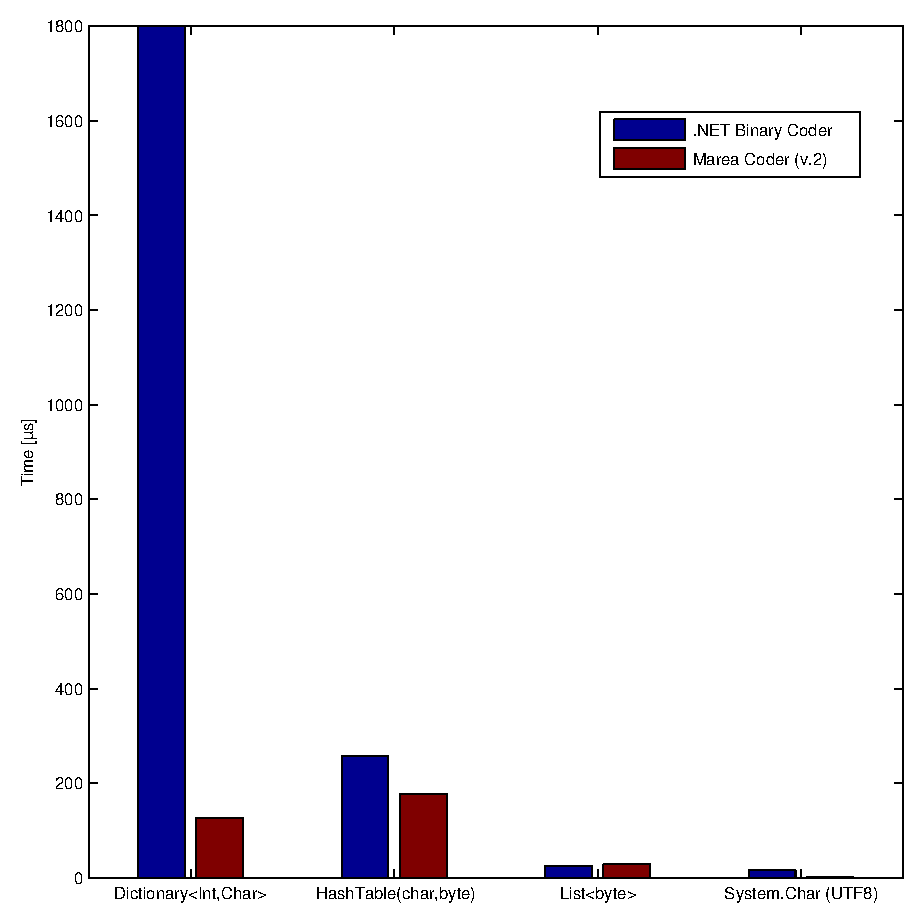
\includegraphics[scale=0.6]{pictures/network/LatencyCoderNewTypes}
  \caption{Encoder layer implementations: Total serialization and deserialization time for new supported types \label{fig:coder-latencies-new-types}}
\end{center}\end{figure}

\section{Transport Layer}\label{S:Transports}

The transport layer provides communication facilities to send and receive data (byte sequences) from the network. This layer provides transfer of data with a certain degree of transparency supporting the two most common transport protocols: TCP and UDP.

TCP transport guarantees reliable end-to-end connection oriented communications. This type of connections require a handshake mechanism in order to negotiate the terms of the connection. The exchange of segments related with this mechanism can adversely affect the performance. 

This problem can be resolved by reusing the established connections instead of opening new TCP connections. The use of persistent connections results in less network traffic, use less time in order to establish new connections and allows the TCP protocol to work more efficiently.

Each MAREA protocol message is sent by TCP transport adding previously a magic number to the corresponding byte sequence representation of itself. This magic number consists in a  synchronization header of 3 bytes followed by an integer (4 bytes) to specify the payload length. The first 3 bytes are use to indicate that the data is synchronized. If this first 3 bytes do not correspond to the expected ones, the transport layer detects that an error condition has happened.

UDP transport provides unreliable (best-effort) datagram comunications. In this type of transport, as the opposite of TCP transport, one stream is opened and closed for the dispatching of each message.

\subsection{Drawbacks}\label{SS:Transports-Drawbacks}

MAREA old transport layer model use the .NET synchronous socket API in order to implement transports. The blocking mode of it set of calls require different threads to accept connections and perform socket I/O operations. 

The use of one thread for each individual connection is non-scalable, especially in Windows systems. The management of a large number of threads is highly inefficient due to the  ineffectiveness of the scheduler to determine which thread should be receiving the processor time. 

The memory overhead is also a handicap. For instance, in Windows the default memory overhead is 1 MB for both native and Common Language Runtime threads.

\subsection{Improvements}\label{SS:Transports-Improvements}

The scalability performance issue can be solved by using asynchronous sockets. Asynchronous I/O operations alleviate the need to create and manage threads \cite{cite:performance-sockets}. This type of sockets use threads internally at the OS Level, which is much faster.

Asynchronous sockets implement specific methods that use  the AsyncCallback class to call completion methods to the following operations: send, receive, connect, accept. Callbacks allow the application to continue processing other events while network operations are been executed.

Two new TCP and UDP asynchronous transport modes have been added in transport layer in order to improve the scalability and the performance.

\subsection{Results}\label{SS:Transports-Results}

Synchronous and asynchronous UDP transports have been compared using a round-trip isolated test. The figure \ref{fig:coder-udp-transports} presents the mean round-trip times during a echo request/response test with simultaneous transports. The mean round-trip time has been calculated according to the average value of the round-trip time of each connection.
 
\begin{figure}[H]\begin{center}
 \centering
  \captionsetup{justification=centering}
  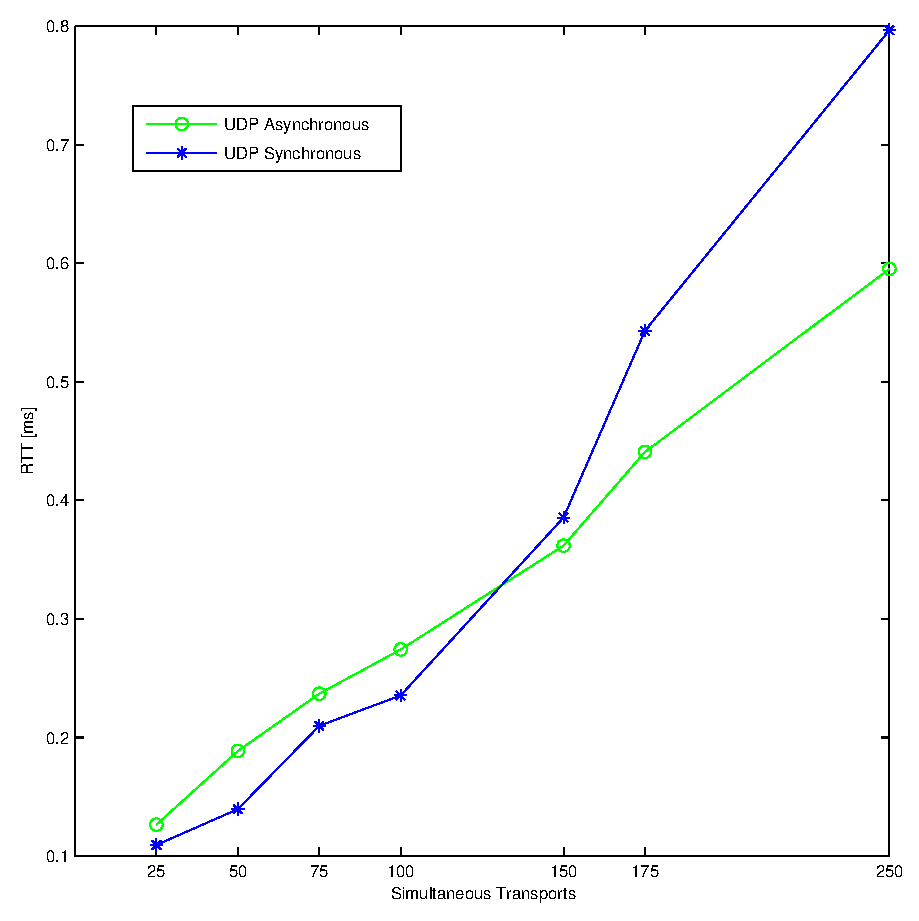
\includegraphics[scale=0.5]{pictures/network/UDPTransports}
  \caption{Mean round-trip times for the echo test using isolated synchronous and synchronous UDP transports (1000 Bytes, 5000 times, 100 Hz) \label{fig:coder-udp-transports}}
\end{center}\end{figure}

According to the results, the round-trip time tends to grow exponentially with the number of simultaneous connections. The round-trip becomes lower in asynchronous mode, in comparison to synchronous mode, from around 150 simultaneous transports. 

\section{MAREA 1 Network Backport}\label{S:MAREA-1-Network-Backport}

The whole new MAREA 2 network architecture has been backported to MAREA 1 in order to ensure its proper functioning. Backporting is the action of taking a certain software modification (patch) and applying it to an older version of the software than it was initially created for \cite{cite:backporting}. This software backport also provides a fair and realistic  way to compare the performance between the old and new network architecture.

\subsection{Results}\label{SS:Backport-Results}

MAREA 1 and MAREA 1 network backport have been compared using a round-trip test. The figure \ref{fig:RRT-backport-UDP} presents the round trip time distribution during a echo request/response test with two MAREA instances. Each instance runs a different service which sends or responds to the messsage. 

The test has been executed 100000 times to send variables (UDP) with a total payload of 1000 bytes and frequency of 100 Hz. The mean round-trip time is 0.2399 and 0.433 ms for MAREA 1 network backport and MAREA 1. The standard deviation is 0.1756 and 0.3813 ms respectively.

\begin{figure}[H]\begin{center}
 \centering
  \captionsetup{justification=centering}
  \includegraphics[scale=0.8]{pictures/network/RTTBackportUDP}
  \caption{Round-trip time distribution for the echo test of MAREA 1 and MAREA 1 network backport using variable primitives (1000 Bytes, 10000 packets, 100 Hz) \label{fig:RRT-backport-UDP}}
\end{center}\end{figure}

The same test has been done using events (TCP). The mean round-trip time is 0.3501 and 0.6564 ms for MAREA 1 network backport and MAREA 1.The standard deviation is 0.2206 and 0.4061 ms respectively.





%\chapter{Protocol Layer}\label{C:Protocol}

\textcolor{red}{//TODO}

\section{Discover Protocol}\label{S:Protocol-Discover}





%%%%%%%%%%%%%%%%%%%%%%%%%%%%%%%%%%%%%%%%%%%%%%%%%%%%%%%%%%%%%%%%%%%%%%%%%
%%%  BIBLIOGRAFIA
%%%%%%%%%%%%%%%%%%%%%%%%%%%%%%%%%%%%%%%%%%%%%%%%%%%%%%%%%%%%%%%%%%%%%%%%%%

%%% Per la bibliografia hi ha 2 opcions: generarla amb la utilitat BibTeX 
%%%                                      o fer-la ''a ma''
%%% NOTA: podeu trobar facilment informaci� sobre BibTeX a:
%%%  http://www.ctan.org/tex-archive/biblio/bibtex/contrib/doc/


%%% OPCIO 1: BibTeX -> descomentar les dues l�nies
%%% a)  Estil de bibliografia\\
%\bibliographystyle{unsrt}  
%%% b) Indicar els fitxers que contenen la bibliografia
%\bibliography{bibliography2}  

%%% OPCIO 2: bibliografia manual
%%%
%%% L'argument d'entrada es el numero de referencies que s'inclouen
\begin{thebibliography}{9}

%% Llibres:  Autor/s (cognoms i inicials dels noms), t�tol del llibre (en cursiva), editor, ciutat i any de publicaci�. Quan es cita el cap�tol d'un llibre s'ha d'indicar el t�tol del cap�tol (entre cometes), el t�tol del llibre (en cursiva) i els n�meros de p�gines amb la primera i la darrera incloses.
%%  Exemple de capitol en llibre

\bibitem{cite:middleware}
Schmidt, D.C. and Schantz, R.E., "Middleware for Distributed System - Evolving the Common Structure for Network-centric Applications", {\it Encyclopedia of Software Eng.}, Wiley \& Sons, New York, 2001. Also available at \url{http://www.agentgroup.unimore.it/didattica/ingss/Lec_Middleware/Schmidt_Middleware.pdf}

\bibitem{cite:mom}
Bagula, A.B., Denko, M.K. and Zennaro, M., "Middleware for Mobile and Pervasive Services", Chap. 7 in {\it Handbook of mobile systems applications and services}, Taylor and Francis Group, Kumar, A. and Xie, B., pp. 248-249, Boca Raton (FL), 2012. 

\bibitem{cite:oom}
Khan, S., Qureshi, K. and Rashid, H., "Performance Comparison of ICE, HORB, CORBA and Dot 
NET Remoting Middleware Technologies", {\it International Journal of Computer Applications}, 3(11), 15-18 (2010). Also available at \url{http://www.ijcaonline.org/volume3/number11/pxc3871105.pdf}

\bibitem{cite:marea}
L�pez, J., Royo, P., Barrado, C., Pastor, E., "Applying marea middleware to UAS communications", {\it  In Proceedings of the AIAA Infotech@Aerospace Conference and AIAA Unmanned Unlimited Conference 2009}, Seattle (WH). Also available at \url{http://upcommons.upc.edu/e-prints/bitstream/2117/9248/1/infotech09.pdf}

\bibitem{cite:thesis-soa-avionics}
L�pez, J., "Service Oriented Architecture for Embedded (Avionics) Applications", {\it  The PhD Program on Computer Architecture Technical School of Castelldefels Technical University of Catalonia}, Barcelona, 2011. Also available at \url{https://dl.dropbox.com/u/2857619/thesis-small.pdf}

\bibitem{cite:delegate}  
Kiely, D., "Delegates Tutorial" in {\it The Microsoft Developer Network (MSDN)}. Available at \url{http://msdn.microsoft.com/en-us/library/aa288459(v=vs.71).aspx}

\bibitem{cite:serialization} 
Albahari, J. and Albahari B., "Serialization", Chap. 17 in {\it C\# 5.0 in a Nutshell: The definitive reference},
O`REILLY, Roumeliotis, R., pp. 691-728, Sebastopol (CA), 2012.

\bibitem{cite:performance-sockets} 
Kiely, D., "Get Closer to the Wire with High-Performance Sockets in .NET" in {\it The Microsoft Developer Network (MSDN) Magazine}. Available at \url{http://msdn.microsoft.com/es-es/magazine/cc300760(en-us).aspx}

\bibitem{cite:backporting}
Books Llc, Source Wikipedia, "Software Quality: Software Crisis, Kludge, Second-System Effect, Workaround, Reliability Engineering, Fault-Tolerant System", Books Llc, Memphis (Tennessee), 2011.

\end{thebibliography}

%%%%%%%%%%%%%%%%%%%%%%%%%%%%%%%%%%%%%%%%%%%%%%%%%%%%%%%%%%%%%%%%%%%%%%%%%%
%%%%%%                           APENDIXS                         %%%%%%%%
%%%%%%%%%%%%%%%%%%%%%%%%%%%%%%%%%%%%%%%%%%%%%%%%%%%%%%%%%%%%%%%%%%%%%%%%%%

\pagestyle{empty}  % no tocar

%% Descomentar una de les dues l�nies seg�ents, en funci� de:
%%  a) els apendixs s'encuadernaran apart (amb portada) 
%%  b) els apendixs s'enquadernen amb el mateix projecte (sense portada). 
%% Recordeu que si tot el document (amb ap�ndixs) excedeix les 100 pagines 
%% s'ha d'enquadernar a part
\appendix\ambportada
%\appendix\senseportada


%%%%%%%%%%%%%%%%%%%%%%%%%%%%%%%%%%%%%%%%%%%%%%%%%%%%%%%%%%%%%%%%%%%%%%%%%%
%%%%%% INCLOURE A PARTIR D'AQUI TOTS ELS CAP�TOLS DELS APENDIXS   %%%%%%%%
%%%%%%%%%%%%%%%%%%%%%%%%%%%%%%%%%%%%%%%%%%%%%%%%%%%%%%%%%%%%%%%%%%%%%%%%%%
\chapter{Technical information. Libraries and Datasheets}\label{C:Libraries-Datasheets}
\section{Library Types}\label{S:appendices-libraries-types}
Below are explained the different types of libraries, its characteristics and the different pros and cons of them.
\begin{itemize}
  \item 
  \textbf{Static Library}
  \\
  This kind of library is that one that is imported while programming, and when the source code is the library is linked statically in the generated binary, this means that the compiler takes the library functions used along the program and then are embedded statically to the compiled binary, in this way, the functions are fiscally located with the program. 
\\
For example, imagine that you create a library with 3 functions, called \verb!get_password()!, \verb!generate_token()! and \verb!hash(char[] plain())!,  but in the current project you only use two of this functions, which are \verb!get_password()! and \verb!get_token()!. When the compiler builds the project code will only take the functions from the library that are currently used in the program and then insert them into the binary. At this point, deleting that library won't affect the generated binary, and it will be able to use it without any dependency problems related to missing libraries (dependencies).
\\
The typical files for this type is .lib for Windows and .a for UNIX systems.
  
  \item
  \textbf{Dynamic Library}
  \\
  In order to avoid the replication of libraries that occurs in static ones, the dynamic libraries were created. This type of libraries is normally used along the operating systems to let applications use the offered functions and APIs written from the OS. In this case, and instead of the functional way of static libraries, any function from the library will be embedded on the generated binary, in this case is important to check that the dependencies are well satisfied when the binary is used, because a missing dependency will break the execution.

In this case, the usual extension files are .dll for Windows and .so for UNIX. But .so files are also used in Windows, especially in web browsers, which use this types of library to load browser plugins such us Flash.

There are two subtypes of dynamic libraries which are explained below:
  \begin{itemize}
    \item 
    \textbf{Dynamically Linked}
  	\\
  	These libraries must be available at compiling/link phase, because the compiler will verify that the function exists and that it is used properly. The libraries will be loaded at start time of the program. In this case, all the functions are mapped into the code.
    \item
    \textbf{Dynamically Loaded}
    \\
    Instead of the previous library, the dynamic loading is used by programs to load or unload libraries and use its functions at run time. When the program needs to use a function it loads the library, then it uses the required functions and finally the library is unloaded again.
    \end{itemize}
\end{itemize}

\textbf{Pros and cons}
\\
The main problem of using static libraries is that the compiled binary takes much more memory and the library is embedded in every program that needs some functions from that library. But, on the other hand, using static libraries the access to its functions by programs is much fast than dynamic ones. Using them also avoids dependency problems, because the dependencies are embedded instead of being located in the file system like dynamic ones.
\\
Regarding the dynamic libraries, they help to avoid replications and memory consumption, and also help to maintain the library updated in all programs that use them, although this can seem pretty good, it can have two bad effects into the generated program. First of all, if the library is missing in the system, the program will not run or will crash in execution time. Secondly, if the library is updated but some methods are changed, the program will crash because the non-existing function, and it will be necessary to readjust the code again, recompile and redistribute it.

\section{spidev.h}\label{S:linux-spi-spidev}
Source code of the library spidev.h used along this project. The different macros needed to configure the ioctl calls.
\begin{lstlisting}[language=C, caption={linux/spi/spidev.h}]
/*
 * include/linux/spi/spidev.h
 *
 * Copyright (C) 2006 SWAPP
 *      Andrea Paterniani <a.paterniani@swapp-eng.it>
 *
 * This program is free software; you can redistribute it and/or modify
 * it under the terms of the GNU General Public License as published by
 * the Free Software Foundation; either version 2 of the License, or
 * (at your option) any later version.
 *
 * This program is distributed in the hope that it will be useful,
 * but WITHOUT ANY WARRANTY; without even the implied warranty of
 * MERCHANTABILITY or FITNESS FOR A PARTICULAR PURPOSE.  See the
 * GNU General Public License for more details.
 *
 * You should have received a copy of the GNU General Public License
 * along with this program; if not, write to the Free Software
 * Foundation, Inc., 675 Mass Ave, Cambridge, MA 02139, USA.
  */

#ifndef SPIDEV_H
#define SPIDEV_H

#include <linux/types.h>

/* User space versions of kernel symbols for SPI clocking modes,
 * matching <linux/spi/spi.h>
 */

#define SPI_CPHA                0x01
#define SPI_CPOL                0x02

#define SPI_MODE_0              (0|0)
#define SPI_MODE_1              (0|SPI_CPHA)
#define SPI_MODE_2              (SPI_CPOL|0)
#define SPI_MODE_3              (SPI_CPOL|SPI_CPHA)

#define SPI_CS_HIGH             0x04
#define SPI_LSB_FIRST           0x08
#define SPI_3WIRE               0x10
#define SPI_LOOP                0x20
#define SPI_NO_CS               0x40
#define SPI_READY               0x80

/*---------------------------------------------------------------------------*/

/* IOCTL commands */

#define SPI_IOC_MAGIC                   'k'

struct spi_ioc_transfer {
        __u64           tx_buf;
        __u64           rx_buf;

        __u32           len;
        __u32           speed_hz;

        __u16           delay_usecs;
        __u8            bits_per_word;
        __u8            cs_change;
        __u32           pad;

        /* If the contents of 'struct spi_ioc_transfer' ever change
         * incompatibly, then the ioctl number (currently 0) must change;
         * ioctls with constant size fields get a bit more in the way of
         * error checking than ones (like this) where that field varies.
         *
         * NOTE: struct layout is the same in 64bit and 32bit userspace.
         */
};

/* not all platforms use <asm-generic/ioctl.h> or _IOC_TYPECHECK() ... */
#define SPI_MSGSIZE(N) \
        ((((N)*(sizeof (struct spi_ioc_transfer))) < (1 << _IOC_SIZEBITS)) \
                ? ((N)*(sizeof (struct spi_ioc_transfer))) : 0)
#define SPI_IOC_MESSAGE(N) _IOW(SPI_IOC_MAGIC, 0, char[SPI_MSGSIZE(N)])


/* Read / Write of SPI mode (SPI_MODE_0..SPI_MODE_3) */
#define SPI_IOC_RD_MODE                 _IOR(SPI_IOC_MAGIC, 1, __u8)
#define SPI_IOC_WR_MODE                 _IOW(SPI_IOC_MAGIC, 1, __u8)

/* Read / Write SPI bit justification */
#define SPI_IOC_RD_LSB_FIRST            _IOR(SPI_IOC_MAGIC, 2, __u8)
#define SPI_IOC_WR_LSB_FIRST            _IOW(SPI_IOC_MAGIC, 2, __u8)

/* Read / Write SPI device word length (1..N) */
#define SPI_IOC_RD_BITS_PER_WORD        _IOR(SPI_IOC_MAGIC, 3, __u8)
#define SPI_IOC_WR_BITS_PER_WORD        _IOW(SPI_IOC_MAGIC, 3, __u8)

/* Read / Write SPI device default max speed hz */
#define SPI_IOC_RD_MAX_SPEED_HZ         _IOR(SPI_IOC_MAGIC, 4, __u32)
#define SPI_IOC_WR_MAX_SPEED_HZ         _IOW(SPI_IOC_MAGIC, 4, __u32)



#endif /* SPIDEV_H */
\end{lstlisting}

\section{SPI Test. RFID Reader}\label{S:linux-spi-spidev}
\subsection{MFRC522 Datasheet}\label{SS:Libs-MFRC522-Datasheet}
The datasheet of this card card reader can be find at the NXP website or in the following link \url{http://www.nxp.com/documents/data_sheet/MFRC522.pdf}.
\\
\subsection{RFID Reader program}\label{SS:Libs-RFID-Reader}
\begin{lstlisting}[language=CSharp, caption={SPIExample.cs - RFID Reading interval}]
using System;
using System.Runtime.CompilerServices;
using System.Threading;
using IOSharp.Utils;
using System.Net;

namespace IOSharp.Exmples
{
    public class SPIExample
    {
        private MFRC522.SPIApi mfrc522 = new MFRC522.SPIApi();
        private bool onUpdate = false;
        private bool activated = false;
        private Timer cardReader = null;

        public static void Main()
        {
            new SPIExample().Run();
        }

        private void Run()
        {
            mfrc522.ConfigureSPI();
            StringUtils.PrintConsole("MF522-AN Version: "+StringUtils.ToHexString(mfrc522.ReadReg_MFRC522(mfrc522.VersionReg)));
            ConfigureTimer(!activated);
            Thread.Sleep(-1);
        }

        private void ConfigureTimer(bool activate)
        {
            if (activate)
            {
                Utils.StringUtils.PrintConsole("****Card reader started****");
                onUpdate = false;
                mfrc522.MFRC522Init();
                cardReader = new Timer(StartMFRC522, this, 0, 500);
                activated = true;

            }
            else
            {
                Utils.StringUtils.PrintConsole("****Card reader stoped****");
                cardReader.Dispose();
                mfrc522.MFRC522Stop();
                activated = false;
            }
        }

        private void StartMFRC522(Object timerInput)
        {
            if (!onUpdate)
            {
                onUpdate = true;
                String cardType = mfrc522.ReadTagTypeString(mfrc522.PICC_REQALL);
                if (!cardType.Equals("*"))
                {
                    CardDetected(cardType, mfrc522.ReadSerialNumberString());
                }
                onUpdate = false;
            }
        }

        private void CardDetected(String cardType, String serialNumber)
        {
            /**Card type
            *			 	0x4400 = Mifare_UltraLight
            *				0x0400 = Mifare_One(S50)
            *				0x0200 = Mifare_One(S70)
            *				0x0800 = Mifare_Pro(X)
            *				0x4403 = Mifare_DESFire
            */

            cardType = cardType.Trim();
            switch (cardType)
            {
                case "44 00":
                    cardType = "Mifare_UltraLight (" + cardType + ") ";
                    break;
                case "04 00":
                    cardType = "Mifare_One(S50) (" + cardType + ") ";
                    break;
                case "02 00":
                    cardType = "Mifare_One(S70) (" + cardType + ") ";
                    break;
                case "08 00":
                    cardType = "Mifare_Pro(X) (" + cardType + ") ";
                    break;
                case "44 03":
                    cardType = "Mifare_DESFire (" + cardType + ") ";
                    break;
            }
            StringUtils.PrintConsole("Card detected: " + cardType + "- Serial: " + serialNumber);
        }
    }
}
\end{lstlisting}

\section{AlterNative System Library}\label{SS:Libs-AlterNative}
\begin{figure}[H]\begin{center}
 \centering
  \captionsetup{justification=centering}
  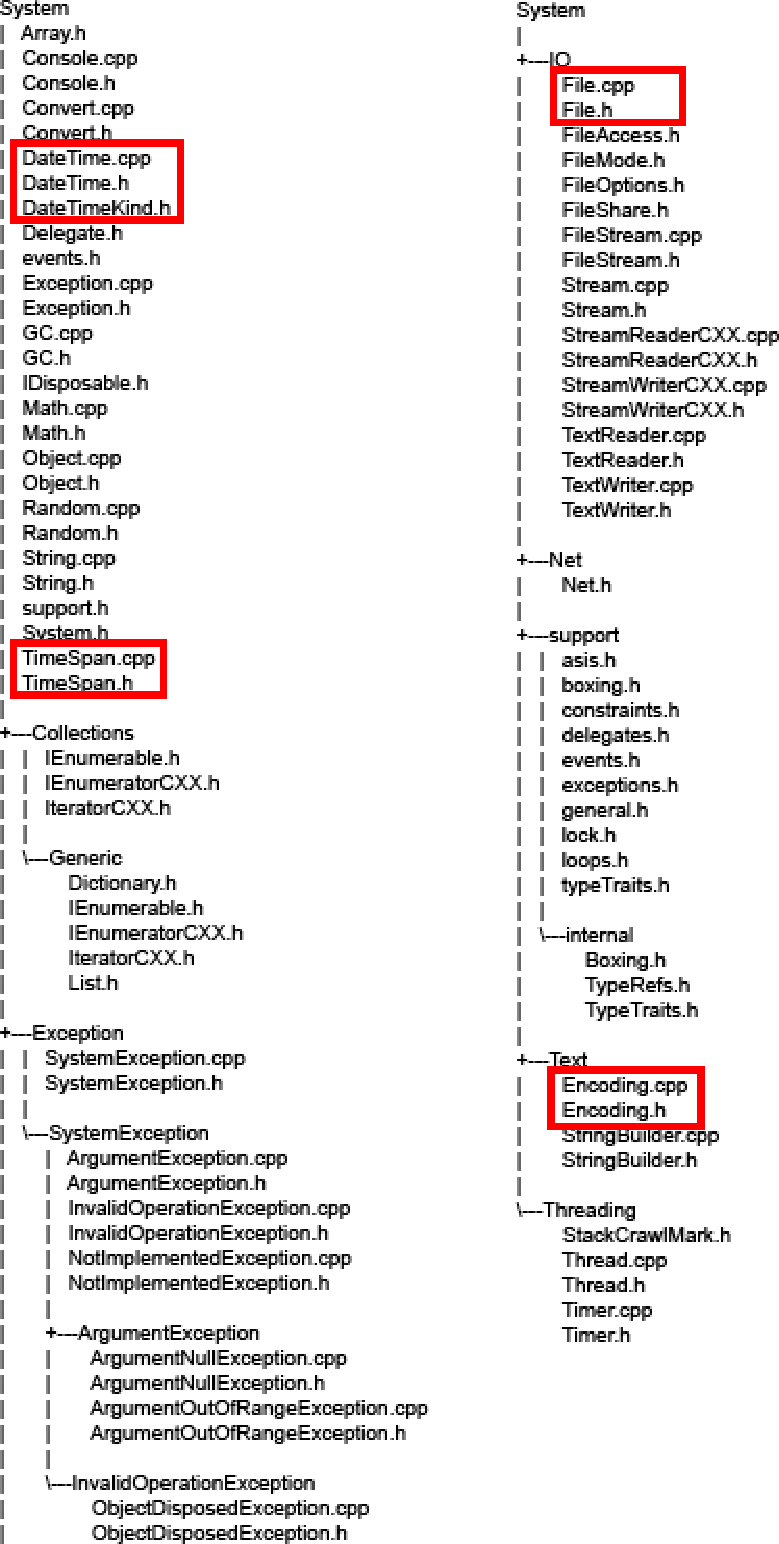
\includegraphics[width=0.75\textwidth]{pictures/appendices/alternative-cpp-classes}
  \caption{Tree dump of the C++ libraries of AlterNative currently implemented\label{fig:Libs-AlterNative}}
\end{center}\end{figure}

\chapter{Exemple de prova d'un ap�ndix}
Text de prova


%%%%%%%%%%%%%%%%%%%%%%%%%%%%%%%%%%%%%%%%%%%%%%%%%%%%%%%%%%%%%%%%%%%%%%%%%%

%%%%%%%%%%%%%%%%%%%%%%%%%%%%%%%%%%%%%%%%%%%%%%%%%%%%%%%%%%%%%%%%%%%%%%%%%%
%%%%%%%%%%%%%%%%%%%%%%%%%%%%%%%%%%%%%%%%%%%%%%%%%%%%%%%%%%%%%%%%%%%%%%%%%%
%%%%%%%%%%%%%%%%%%%%%%%%%%%%%%%%%%%%%%%%%%%%%%%%%%%%%%%%%%%%%%%%%%%%%%%%%%
% i  aixo es tot! ;)
\end{document}





